\documentclass[11pt]{beamer}
\usepackage[UTF8]{ctex}
\usepackage[utf8]{inputenc}
\usepackage[T1]{fontenc}
\usepackage{lmodern}
\usepackage{amsmath}
\usepackage{amsfonts}
\usepackage{amssymb}
\usepackage{graphicx}
\usepackage{chronology}
\usetheme{CambridgeUS}

\usepackage{pdfpages}
%%%%%
\usepackage{longtable}
\usepackage{subfigure}
\usepackage{color}
\usepackage{booktabs}

%% LOGO放右上
\setbeamertemplate{frametitle}
{\begin{beamercolorbox}[wd=\paperwidth]{frametitle}
		\strut\hspace{0.5em}\insertframetitle\strut
		\hfill
		\raisebox{-2mm}{
\includegraphics[width=1cm]{figures/HNUC.jpeg}}
	\end{beamercolorbox}
}

\begin{document}
\author{郭泰彪}
\title{区块链原理及应用}
\subtitle{第2课:区块链的发展历程快速回顾\footnote{不推荐投资加密货币,谨防上当受骗。}}
\institute{湖南工商大学大数据与互联网创新研究院}
\date{2020年9月17日}

\begin{frame}[plain]
	\maketitle
\end{frame}

\begin{frame}[shrink]
	\frametitle{目录}
	\tableofcontents[sectionstyle=show,subsectionstyle=show/shaded,subsubsectionstyle=show/shaded]
\end{frame}

\section{比特币的燃情岁月:区块链1.0}

\subsection{比特币趣事两则}
\begin{frame}{如果大三学生的你有6000元,该投资什么}
	\begin{figure}
		\centering
		{\Huge 如果你有6000元,投资什么?}
	\end{figure}
\end{frame}

\begin{frame}{知乎19982269号问题}

	大三的学生,手头有6000元的钱,想要做些小投资赚点儿钱,有什么好建议么?

	\footnotesize{这是除去学费和生活费之后的,所以觉得就存在银行里没什么用,想利用这些钱去做点投资。}
\end{frame}

\begin{frame}{知乎19982269号问题}
	\begin{figure}
		\centering
		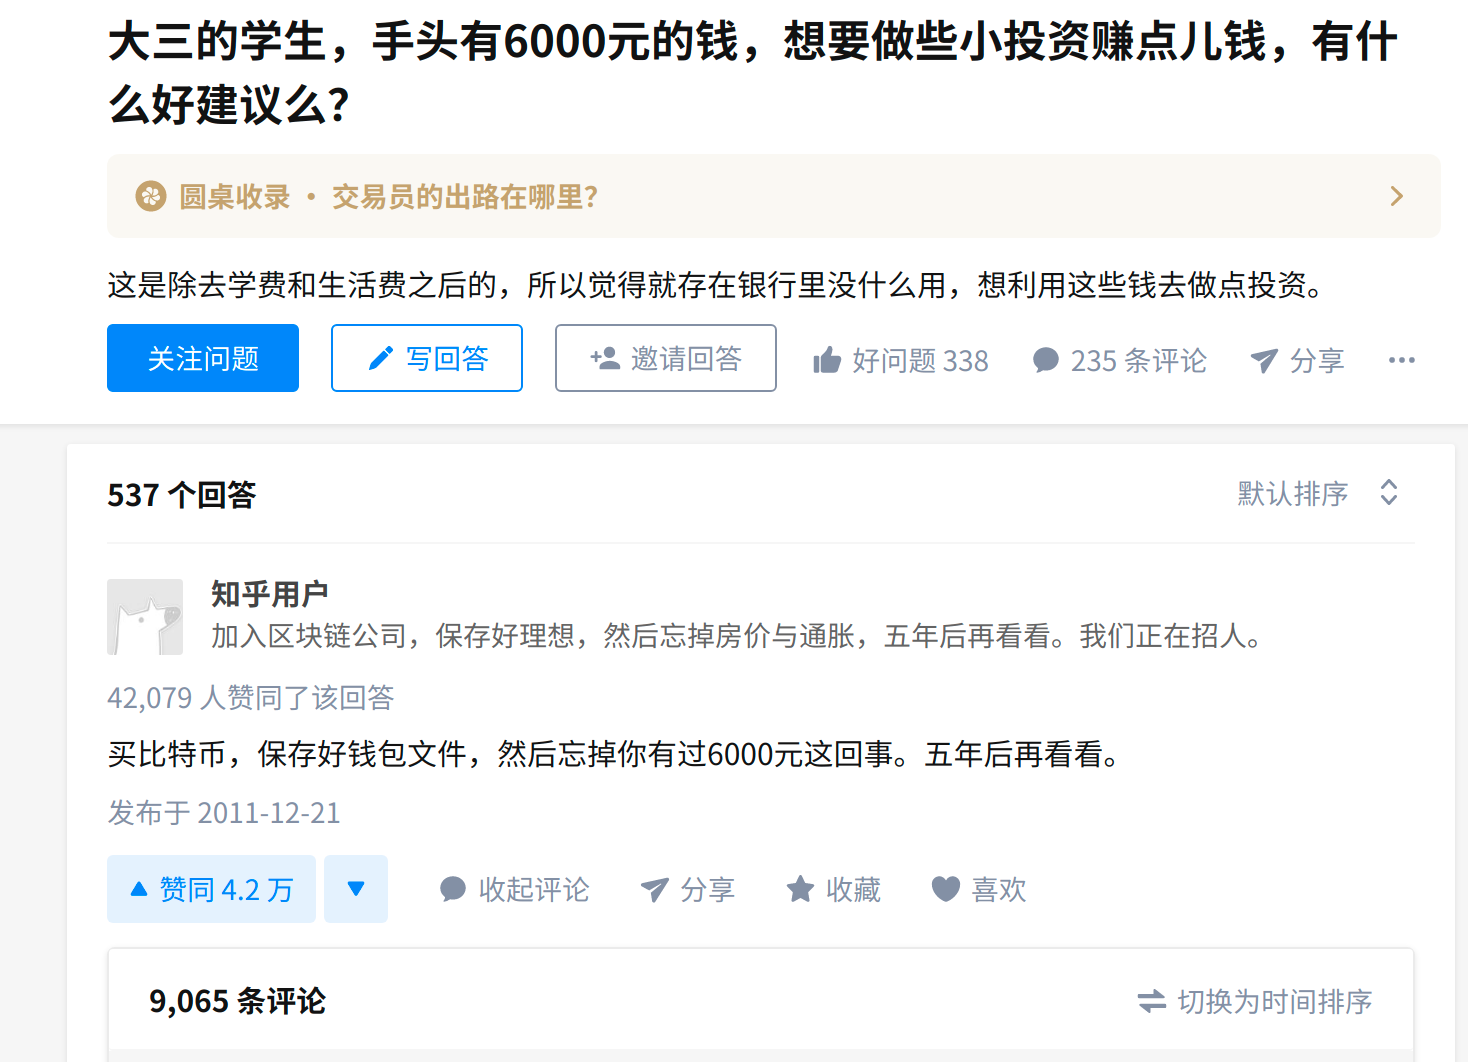
\includegraphics[width=0.8\linewidth]{figures/zhihu19982269}
		\label{fig:zhihu19982269}
	\end{figure}
\end{frame}

\begin{frame}{知乎19982269号问题}
	\begin{figure}
		\centering
		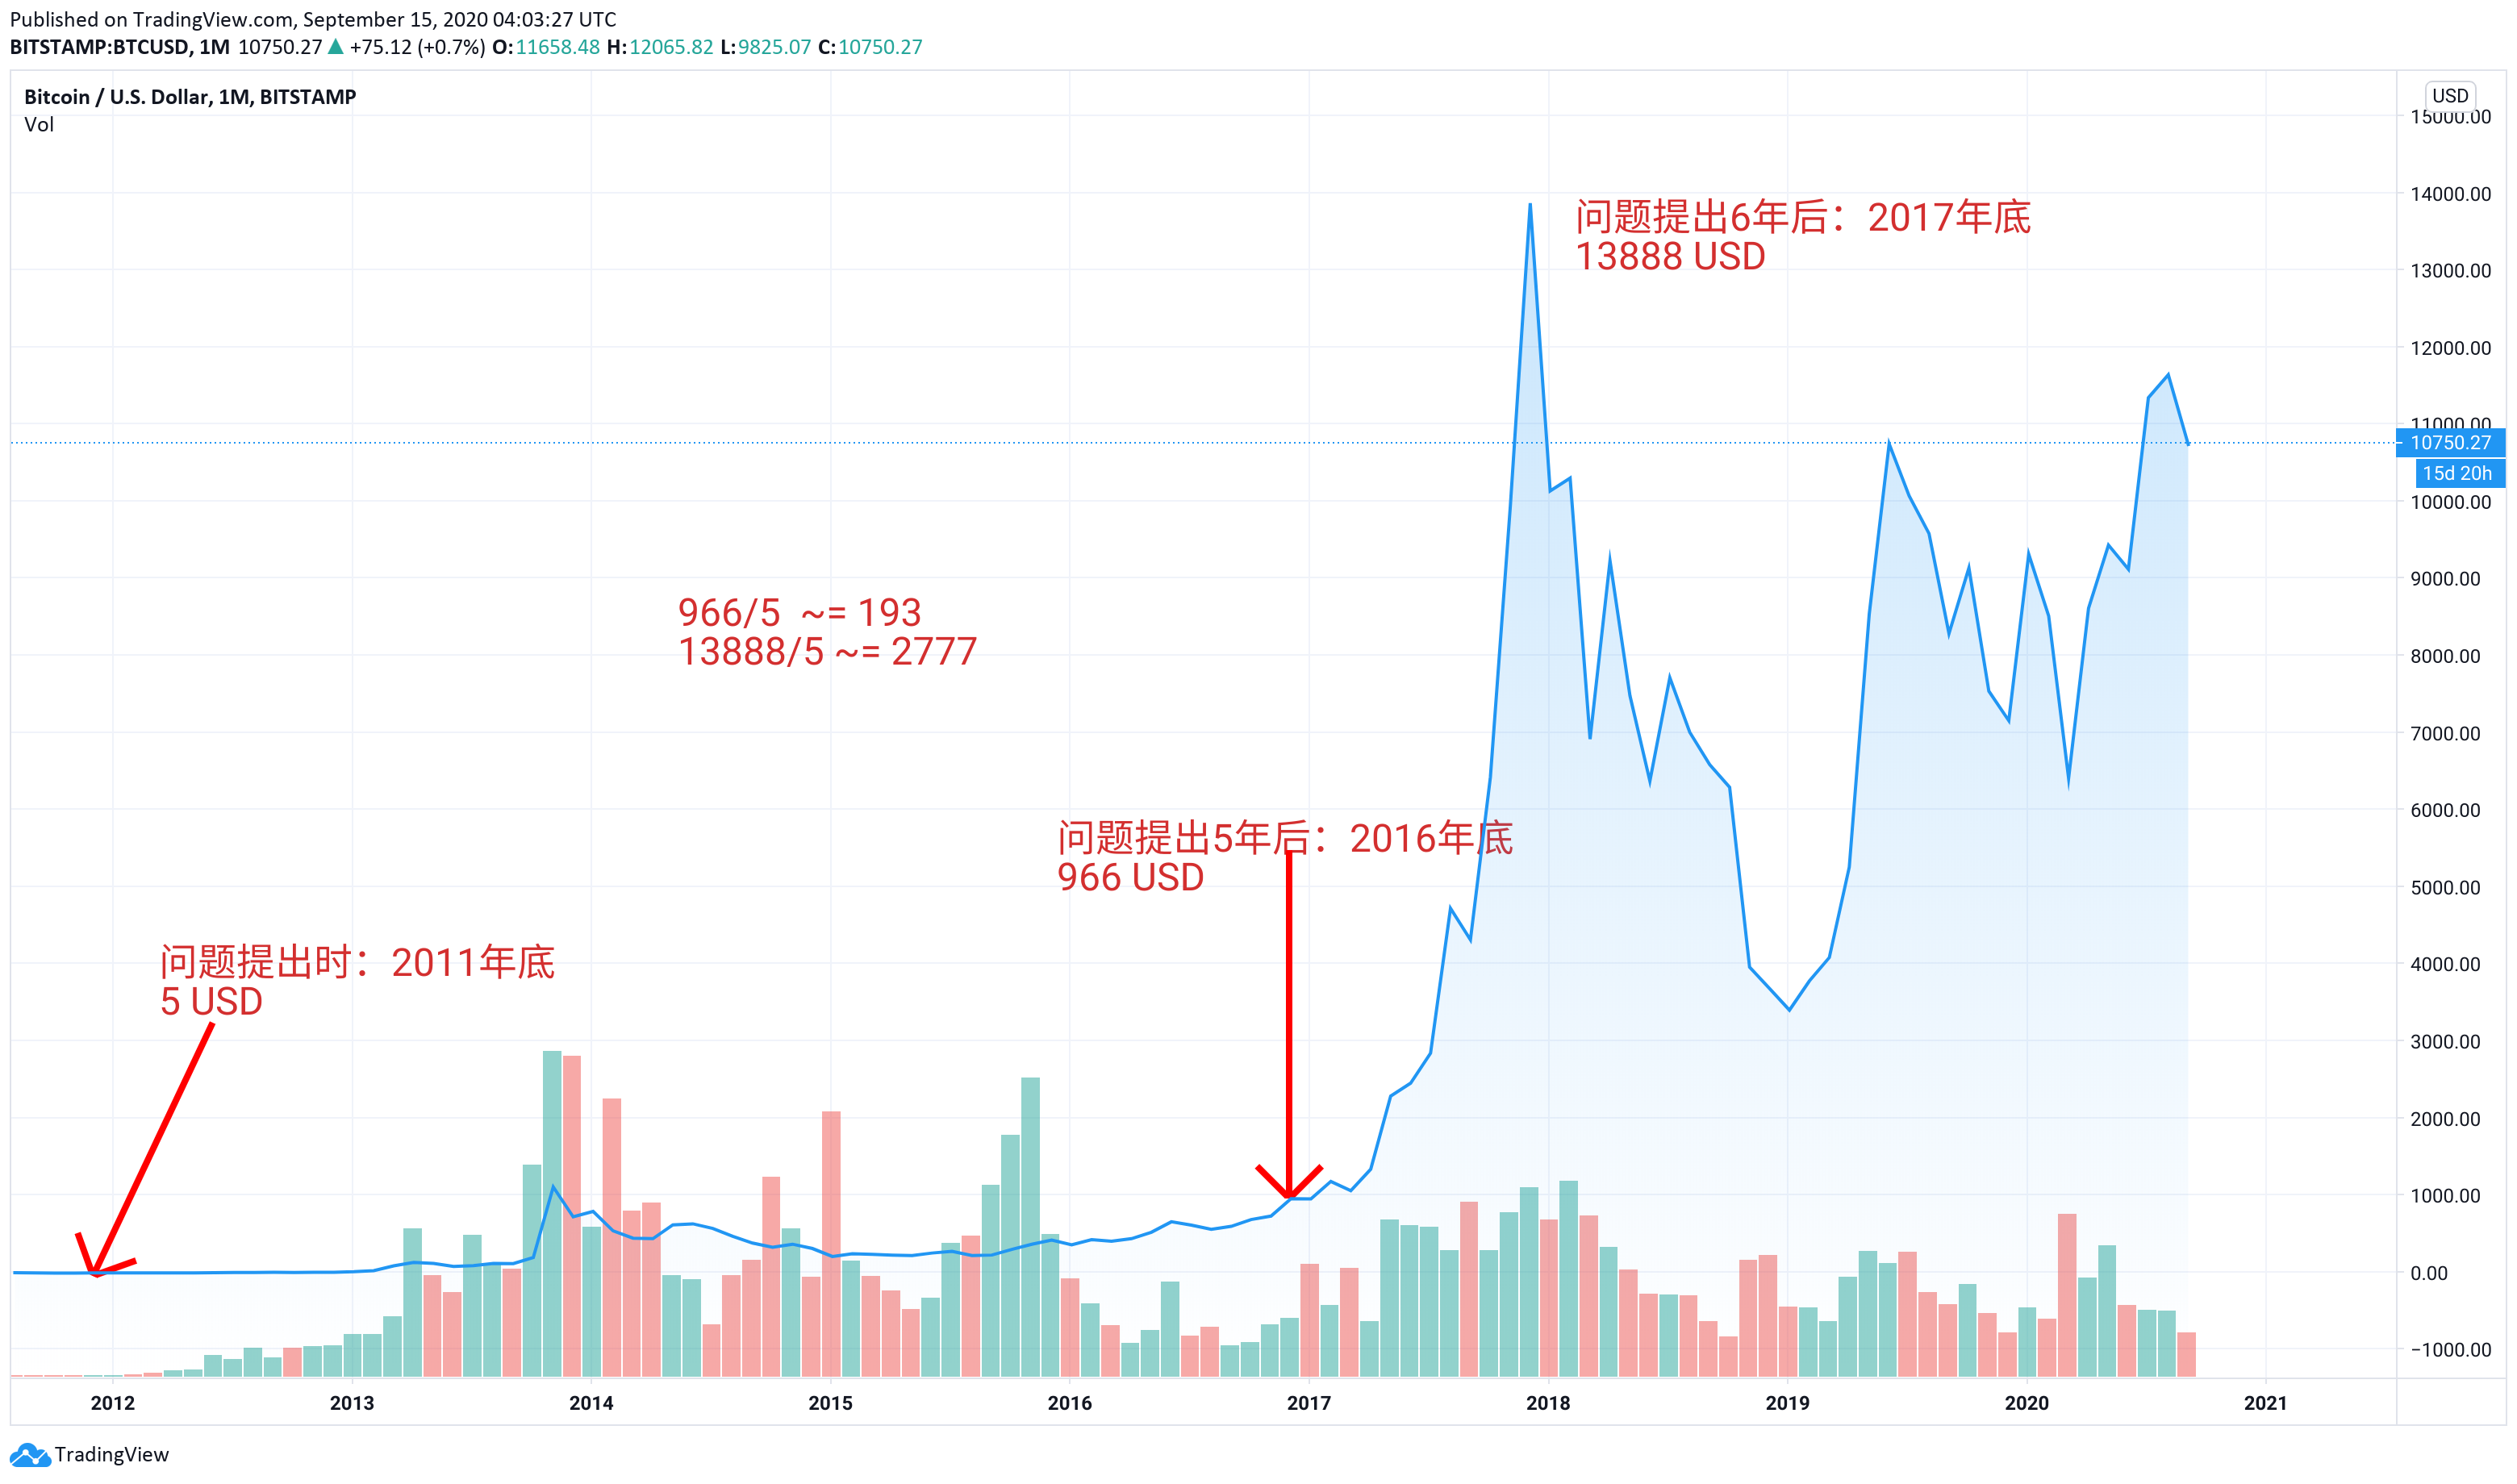
\includegraphics[width=\linewidth]{figures/btc6000}
	\end{figure}
\end{frame}

\begin{frame}{比特币点外卖,三天才送到}
	翻译: 我想要2块大披萨,希望能用10000枚比特币来换。披萨可以是从商店购买的,也可以是自制的。但是我需要你把披萨送到我的家门口,就像酒店的餐饮服务一样,不需要我自己准备并购买。我喜欢洋葱、胡椒、香肠和蘑菇,不要奇怪的鱼肉披萨!
	\begin{figure}
		\centering
		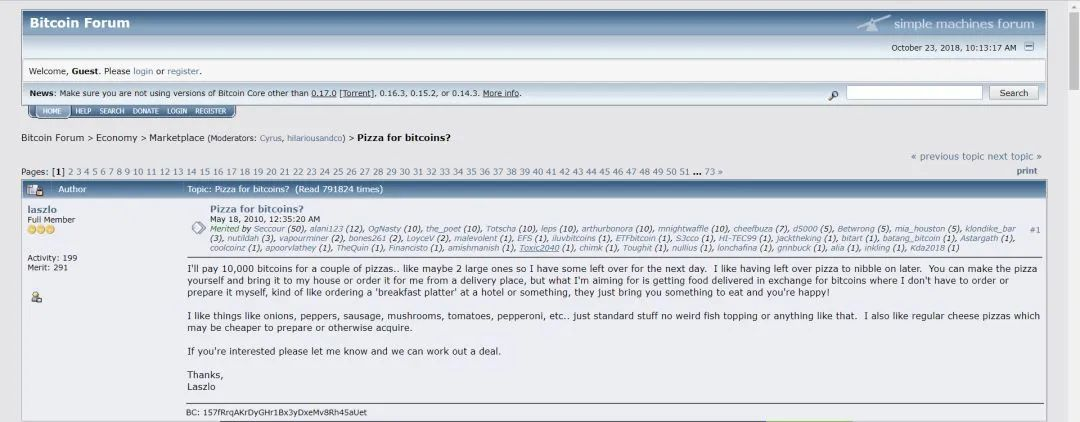
\includegraphics[width=0.7\linewidth]{figures/pizzabbs}
		\caption{比特币论坛帖子截图}
		\label{fig:pizzabbs}
	\end{figure}
\end{frame}

\begin{frame}[allowframebreaks]{Hanyecz买披萨时的截图}
	\begin{figure}
		\centering
		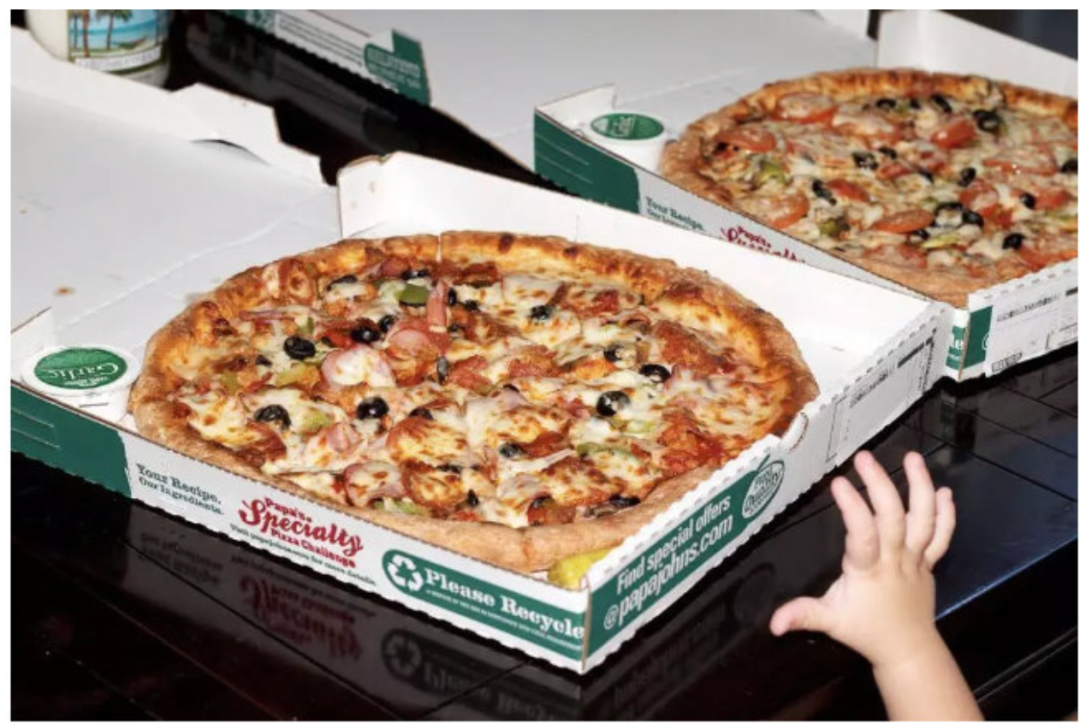
\includegraphics[width=0.7\linewidth]{figures/pizza01}
		\caption{世界上最"贵"的两块披萨}
	\end{figure}

	\begin{figure}
		\centering
		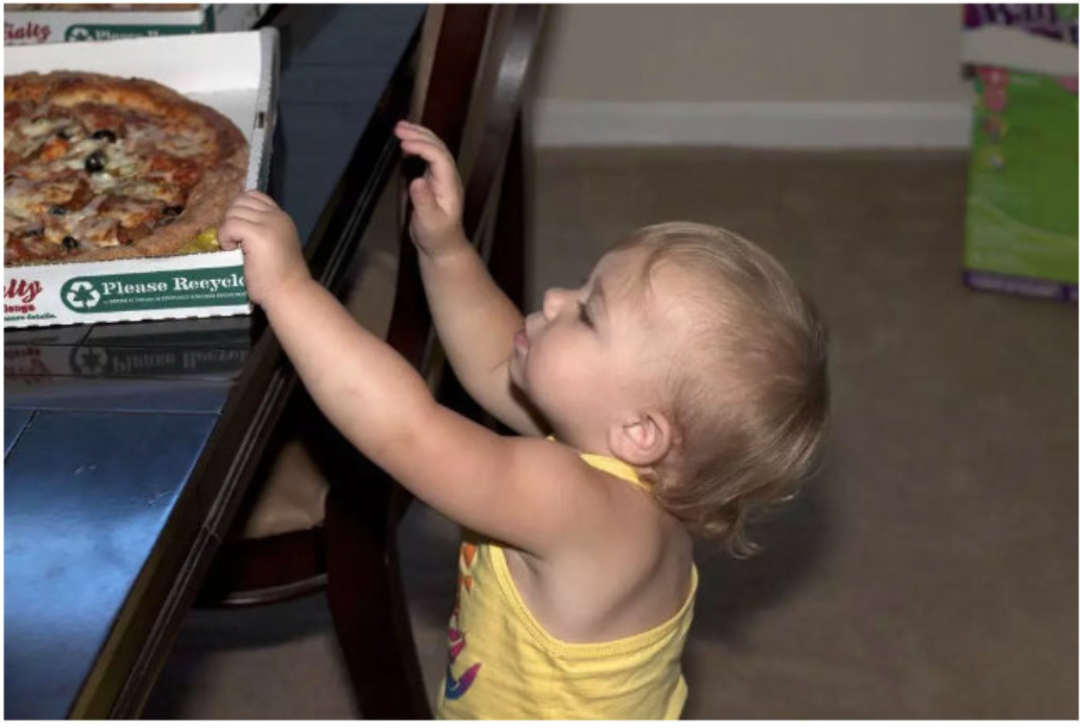
\includegraphics[width=0.7\linewidth]{figures/pizza02}
		\caption{Laszlo表示自己1岁的女儿不是用比特币换的}
	\end{figure}

	\begin{figure}
		\centering
		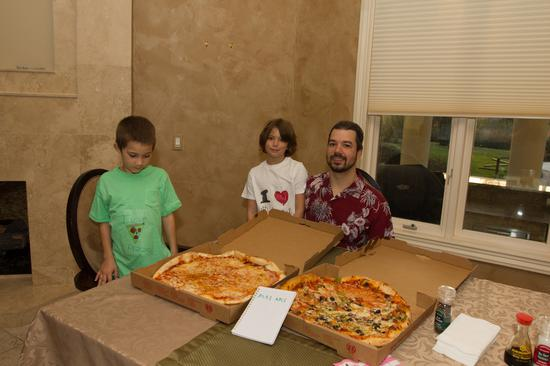
\includegraphics[width=0.6\linewidth]{figures/pizzabybtc}
		\caption{Laszlo在交易完成后还上传了自己与家人共同享用披萨的照片,有趣的是他的一个孩子穿着印有“我爱披萨”字样的衣服,另一个孩子穿着印有“我爱比特币”的衣服}
		\label{fig:pizzabybtc}
	\end{figure}

\end{frame}

\subsection{挖矿的军备竞赛}
\begin{frame}{挖矿的军备竞赛}
	Laszlo 为什么拥有这么多比特币?

	比特币购买披萨的主人公是GPU挖矿第一人。(2010年)
\end{frame}

\begin{frame}{从CPU到ASIC}
	\begin{figure}
		\centering
		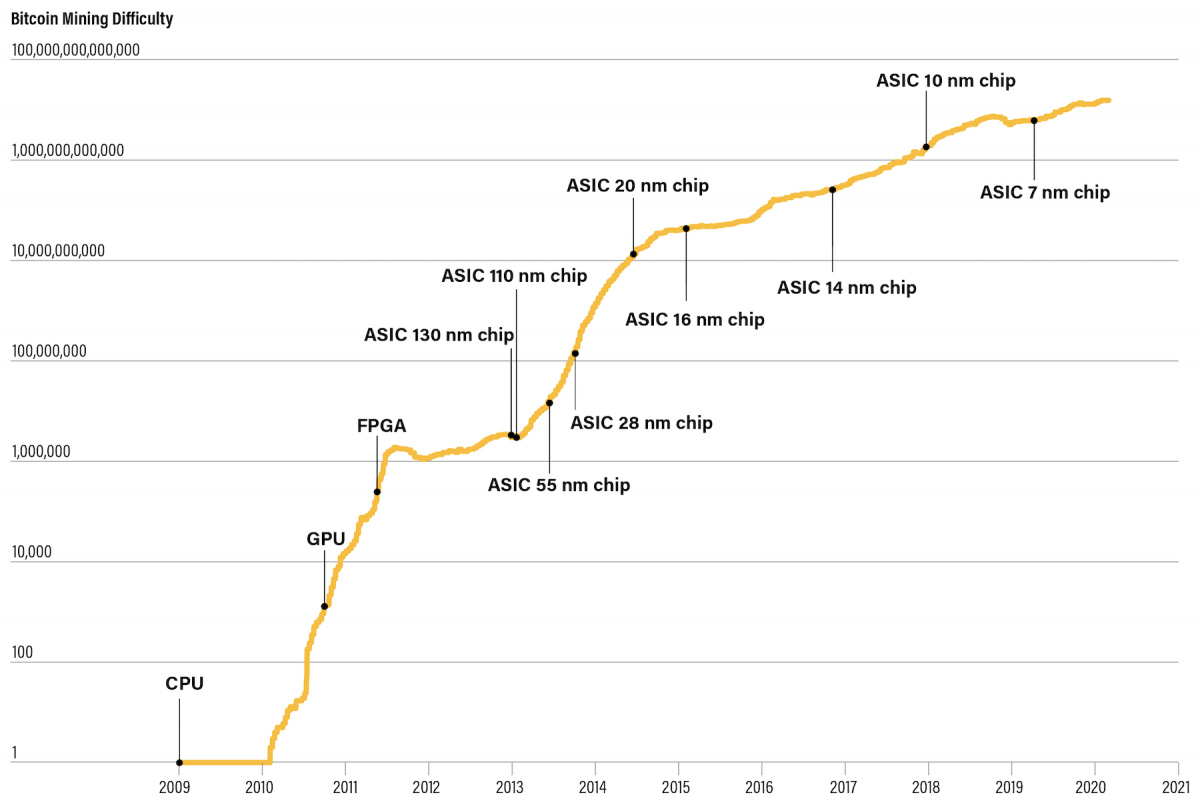
\includegraphics[width=0.8\linewidth]{figures/deviceRevolutionWithPrice}
		\caption{比特币挖矿设备进化速度和比特币挖矿难度关系}
		\label{fig:devicerevolutionwithprice}
	\end{figure}
\end{frame}

\begin{frame}{从CPU到ASIC}
	\begin{figure}
		\centering
		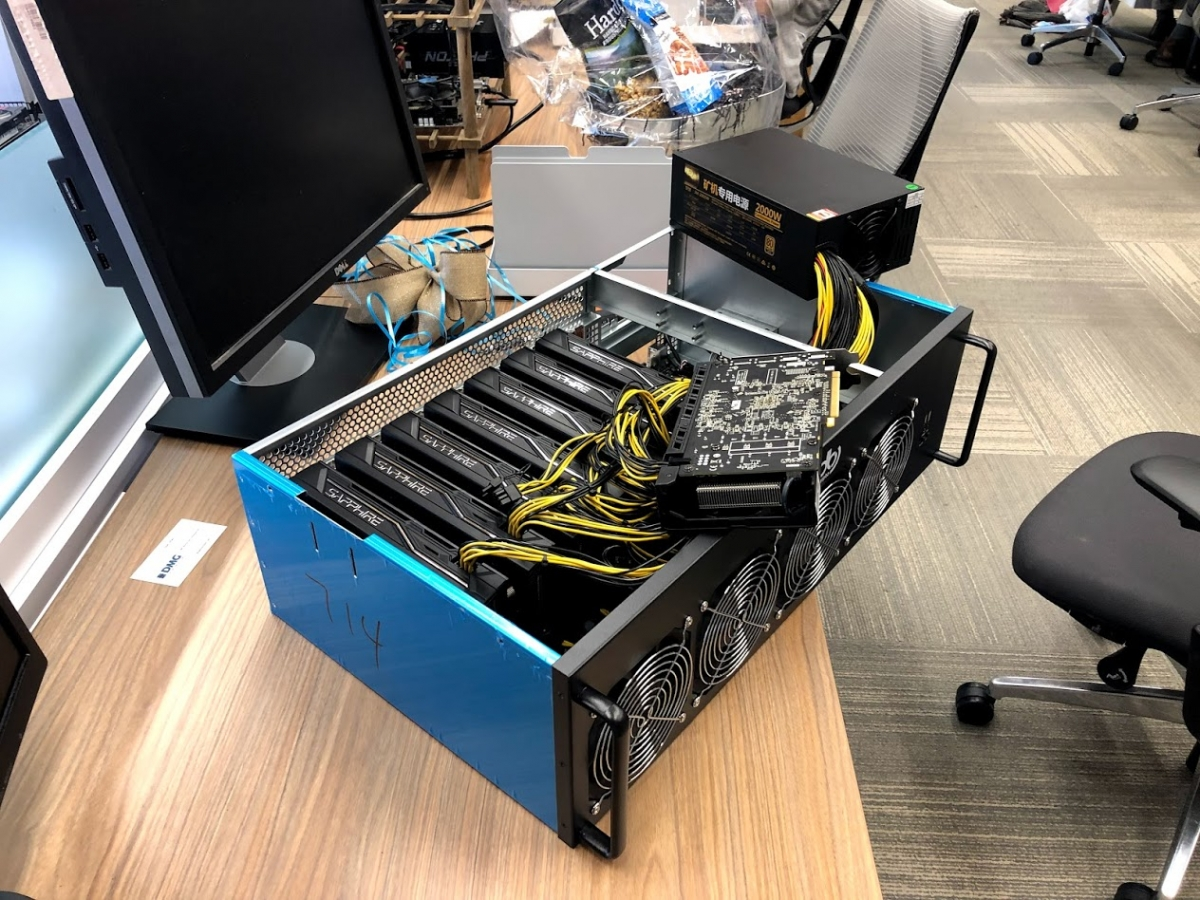
\includegraphics[width=0.7\linewidth]{figures/GPUMining}
		\caption{多路GPU矿机}
	\end{figure}
\end{frame}

\begin{frame}{从CPU到ASIC}
	\begin{figure}
		\centering
		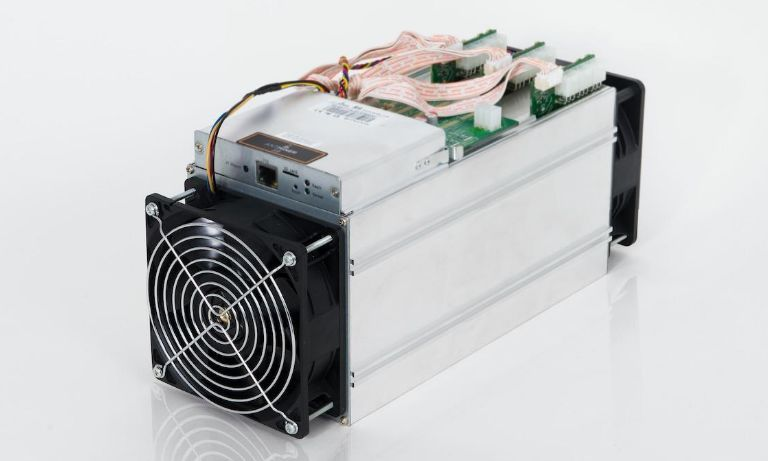
\includegraphics[width=0.7\linewidth]{figures/ASICMining}
		\caption{ASIC矿机}
	\end{figure}
\end{frame}

\begin{frame}{CPU、GPU、FPGA、ASIC挖矿性能对比}

	% Please add the following required packages to your document preamble:
	% \usepackage{booktabs}
	% \usepackage{graphicx}
	\begin{table}[]
		\centering
		\resizebox{0.8\textwidth}{!}{%
			\begin{tabular}{@{}p{0.25\linewidth}p{0.25\linewidth}p{0.25\linewidth}p{0.25\linewidth}@{}}
				\toprule
				                             & CPU            & GPU                      & ASIC                   \\ \midrule
				适用场景                     & 通用计算       & 半通用计算,适合图像处理 & 专用计算,针对特点算法 \\
				代表产品                     & Intel i7 2600k & GTX 1080                 & Antminer s9i           \\
				价格(\$)                     & 316            & 800                      & 794                    \\
				针对SHA256算法的算力(GH/Z) & 0.02           & 2.8                      & 14000                  \\
				功耗(W)                      & 120            & 300                      & 1375                   \\
				单位算力功耗(W/GHs)          & 6000           & 107                      & 0.098                  \\
				单位算力价格(\$/GHs)         & 15800          & 286                      & 0.06                   \\ \bottomrule
			\end{tabular}%
		}
		\caption{CPU、GPU、ASIC挖矿性能对比\footnote{资料来源:en.bitcoin.it、比特大陆官网、github、国盛证券研究所}}
		\label{tab:my-table}
	\end{table}
\end{frame}

\subsection{比特币矿池}
\begin{frame}{单机挖矿到矿池挖矿}
	比特币挖矿规则:大约7分钟出一个区块,某个矿工得到所有的奖励,算力越高的矿工得到奖励的几率越大。两种挖矿的模式:
	\begin{enumerate}
		\item 个人挖矿(Solo){\color{red} 欧皇适用}:
		      \begin{itemize}
			      \item 比特币初期流行的挖矿方式;
			      \item 但随着比特币挖矿人数变多,算力增加,收益变得不稳定;
		      \end{itemize}
		\item 矿池挖矿(Stake Pool){\color{red} 非酋适用}:
		      \begin{itemize}
			      \item 现在比特币主流的挖矿方式;
			      \item 将大家算力集中起来,将挖到的比特币进行平分,收益稳定;
		      \end{itemize}
	\end{enumerate}
	\begin{align}
		E_{solo}      & =E_{stake}       \\
		\sigma_{solo} & >=\sigma_{stake}
	\end{align}
\end{frame}

\begin{frame}{矿池收益结算模式}
	\begin{enumerate}
		\item  PPS(Pay Per Share):
		      \begin{enumerate}
			      \item 根据你share的任务量进行计算,{\color{red}收益恒定};
			      \item $gain_{worker}=C\times Power,gain_{pool}=X-n\times gain_{worker}$
			      \item 类似打工,你把劳动力卖给矿池获得固定收益,矿池自负盈亏;
		      \end{enumerate}
		\item PPLNS(Pay Per Last N Shares):
		      \begin{enumerate}
			      \item 根据你的股份比重来分配收益,{\color{red}收益短期内有波动};
			      \item 每个时间片内矿池获得的比特币数量不同,根据在每个时间片内你股份比例分配收益;
			      \item 幸运值公式 $Lucky = \frac{RealGain}{TheoryGain}\times 100 \%$
		      \end{enumerate}
	\end{enumerate}
\end{frame}

\begin{frame}{矿池的中心化风险}
	比特币算力集中在一小部分人手中很有可能会危及比特币的系统安全,从而引发比特币的经济系统崩溃和作恶的情况发生。

	\begin{figure}
		\centering
		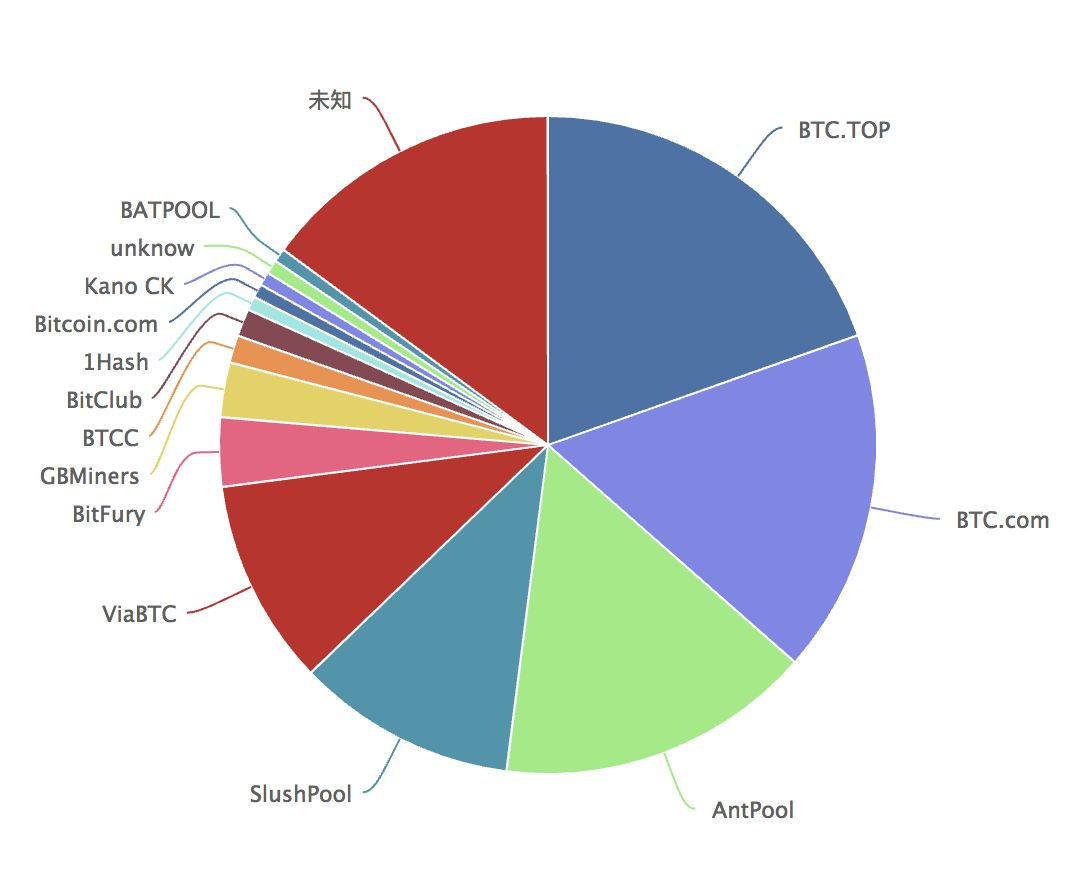
\includegraphics[width=0.45\linewidth]{figures/poolPie}
		\caption{前三公有矿池如果被操纵就具备超过51\%的算力\footnote{51\%攻击揭示了超过50\%的算力被恶意用户操纵的话比特币的记录就存在被操纵和篡改的风险。}。}
		\label{fig:poolpie}
	\end{figure}

\end{frame}

\subsection{比特币矿场}

\begin{frame}{全球加密货币矿场分布图}
	比特币矿场7成来自中国,其中4成在四川(2017年数据)。
	\begin{figure}
		\centering
		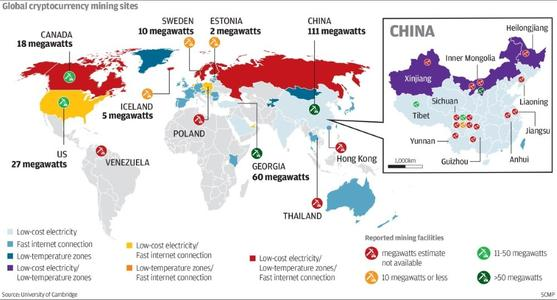
\includegraphics[width=0.9\linewidth]{figures/globalCryptocurrencyMiningMap}
		\caption{全球加密货币挖矿分布图}
		\label{fig:globalcryptocurrencyminingmap}
	\end{figure}
\end{frame}

\begin{frame}{矿场实景图}
	\begin{figure}
		\centering
		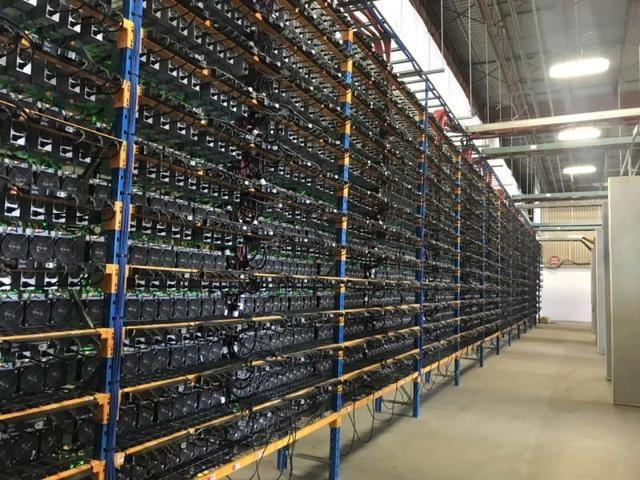
\includegraphics[width=0.7\linewidth]{figures/miningFactory}
		\caption{矿场内部的场景,密密麻麻的矿机}
		\label{fig:miningfactory}
	\end{figure}
\end{frame}

\begin{frame}{比特币挖矿能耗惊人}
	\begin{figure}
		\centering
		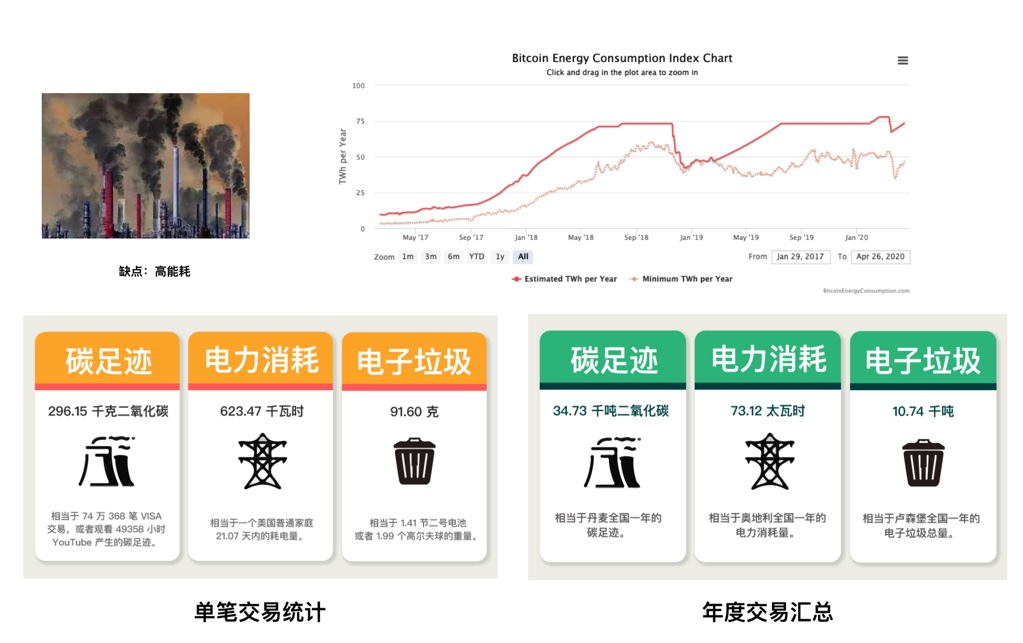
\includegraphics[width=0.88\linewidth]{figures/powerWastedOfBTCjpg}
		\label{fig:powerwastedofbtcjpg}
	\end{figure}

\end{frame}
\subsection{比特币交易方式演变}
% 面对面交易至交易所

\begin{frame}{面对面交易}
	最原始的比特币的交易方式,对于黑产等因为KYC和反洗钱无法通过正规交易所的交易来说仍然非常有效。
	\begin{figure}
		\centering
		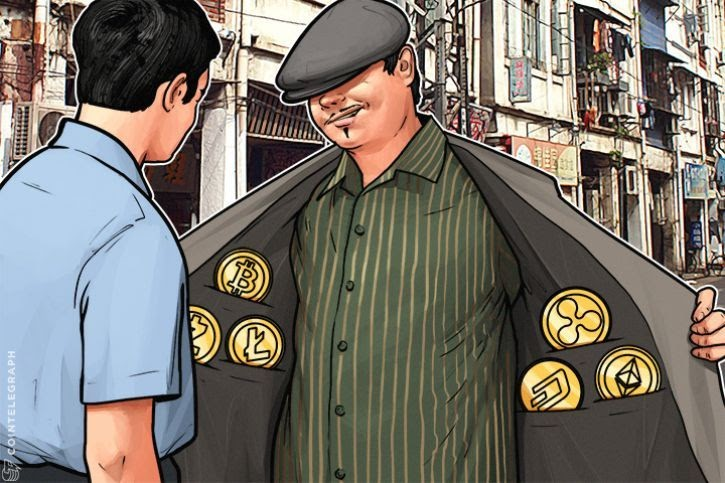
\includegraphics[width=0.6\linewidth]{figures/btcFaceToFace}
		\caption{加密货币,一块钱四个,嘿嘿}
		\label{fig:btcfacetoface}
	\end{figure}

\end{frame}

\begin{frame}{交易所}
	提供了加密货币价格展示、加密货币间交易、加密货币衍生品交易。

	大部分都不支持中国地区,部分国家承认其合法性。
	\begin{itemize}
		\item 币币交易;
		\item 法币加密货币交易;
		\item 合约交易(DiFi等金融衍生品);
		\item 平台币;
	\end{itemize}

	\begin{figure}
		\centering
		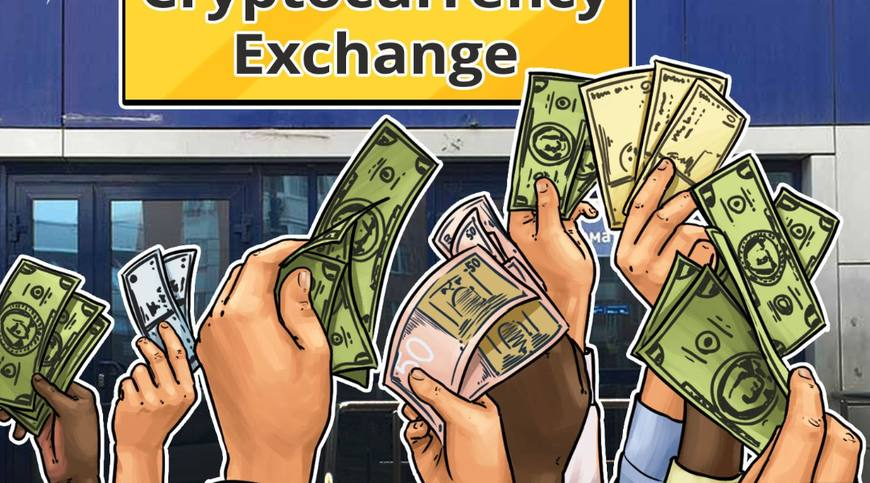
\includegraphics[width=0.6\linewidth,height=0.4\textheight]{figures/exchange}
		\caption{加密货币交易所}
		\label{fig:exchange}
	\end{figure}

\end{frame}

\begin{frame}{加密货币信用卡、ATM}

	\begin{minipage}[t]{0.5\linewidth}
		\centering
		\begin{enumerate}
			\item 加密货币信用卡可以在日常消费中使用加密货币进行支付;
			\item 加密货币ATM可以使用加密货币兑换现金,或进行加密货币的转账等;
			\item 澳洲、欧洲对加密货币信用卡、ATM支持度较高。
		\end{enumerate}

	\end{minipage}%
	\begin{minipage}[t]{0.4\linewidth}
		\begin{figure}
			\centering
			\subfigure[加密货币信用卡]{
				\begin{minipage}[b]{0.8\linewidth}
					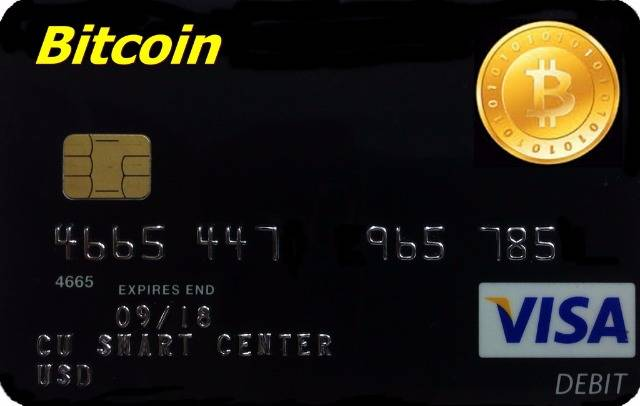
\includegraphics[width=\linewidth]{figures/btcVisaCard}
				\end{minipage}%
			}
			\subfigure[加密货币ATM]{
				\begin{minipage}[b]{0.8\linewidth}
					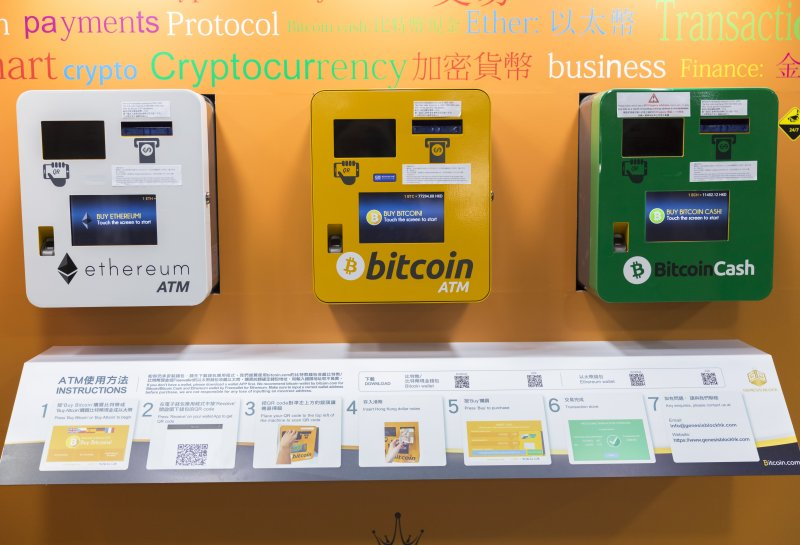
\includegraphics[width=\linewidth]{figures/bitcoinAtm}
				\end{minipage}%
			}
		\end{figure}
	\end{minipage}%
\end{frame}

\subsection{比特币金融衍生品}

\begin{frame}{常见比特币金融衍生品}
	\begin{minipage}[t]{0.7\linewidth}
		\footnotesize
		\begin{enumerate}
			\item 期货类:期货合约是期货交易所制定的标准化合约,对合约到期日及其买卖的资产的种类、数量、质量作出了统一规定。
			      \begin{enumerate}
				      \item 火币、OkEx、BitMEX等从交割合约的基础上衍生出永续合约;
				      \item 芝加哥商品交易所CME和芝加哥期权交易所CBOE等;
			      \end{enumerate}
			\item 期权类:期权交易是买卖权利的交易。期权合约规定了在某一特定时间、以某一特定价格买卖某一特定种类、数量、质量原生资产的权利;
			      \begin{enumerate}
				      \item 芝加哥商品交易所CME推出比特币期权;
			      \end{enumerate}
			\item 去中心化金融 DiFi:区块链和智能合约设计金融产品;
			\item 稳定币;
		\end{enumerate}
	\end{minipage}%
	\begin{minipage}[t]{0.3\linewidth}
		\begin{figure}
			\centering
			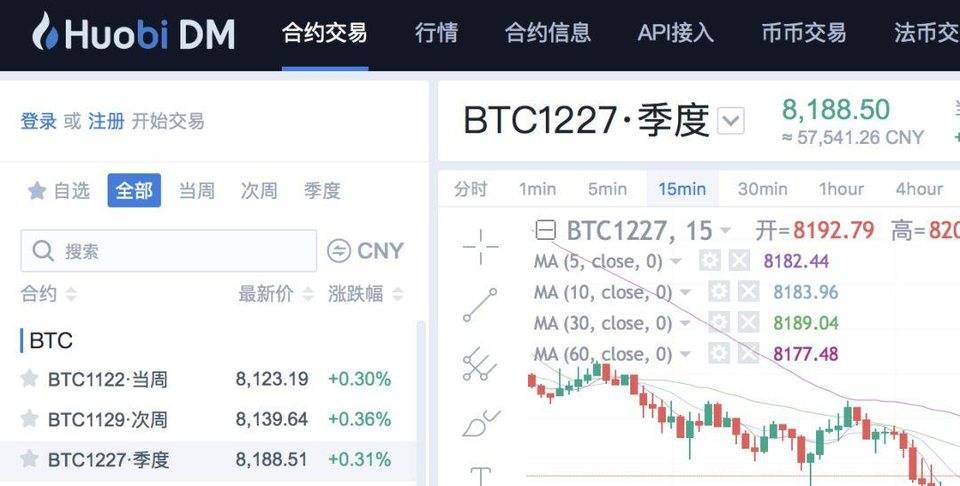
\includegraphics[width=\linewidth]{figures/ccContracts}
			\caption{火币合约交易截图}
		\end{figure}
	\end{minipage}%
\end{frame}

\section{智能合约和ICO狂潮:区块链2.0}
\subsection{智能合约对区块链的意义}
\begin{frame}{智能合约定义}

	\begin{enumerate}
		\item 智能合约(Smart contract)是一种旨在以信息化方式传播、验证或执行合同的计算机协议。智能合约允许在没有第三方的情况下进行可信交易,这些交易可追踪且不可逆转;
		\item 提出者: 尼克·萨博(密码朋克成员,法学博士,中本聪候选人) 1995年;
		\item 定义:智能合约是一种计算机化的交易协议,可以执行合同的条款。
		      {\footnotesize 一般的目的是满足常见的契约条件(例如支付条款、扣押权、机密性、甚至是强制执行),将恶意攻击和意外情况降低至最小,并最小化对受信中介的需求。相关的经济目标包括降低欺诈损失、仲裁和执行成本,以及其他交易成本。}
	\end{enumerate}

\end{frame}

\begin{frame}{智能合约的性质}

	\begin{enumerate}
		\item \textbf{智能合约是计算机程序}

		      {\tiny 智能合约是一种安全的、处于运行状态的计算机程序。智能合约实际上是采用某种语言编写的,计算机可以理解的代码。智能合约的内容是包含了业务逻辑和各方间约定好的协议。}

		\item \textbf{智能合约能自动执行}

		      {\tiny  智能合约和运行在单机上的计算机程序的不同点在于当满足约定的条件时,智能合约将会自动执行履行契约(以以太坊为例,智能合约实际实现时不是自动运行的,而是由用户主动驱动的)。自动执行意味着智能合约将按照规定的路线完成合约内容,并返回合约的执行结果。合约的去中介化,合约条款的自动执行成为可能,合约的自动执行减少了合约参与者的成本。}

		\item \textbf{智能合约的执行不可阻挡}

		      {\tiny  智能合约的执行具有不可阻挡性,只要满足约定的条件,合约将自动执行且不能被打断。这体现了“代码即法律”的理念,现实社会中的合约信度由法律和国家做背书,但在智能合约中由智能合约的不可阻挡性做背书,点对点的交易双方不再需要一个中介机构来做担保。除非关闭所有区块链节点,否则智能合约就可以被正确执行。}

		\item \textbf{智能合约的执行结果具有确定性}

		      {\tiny  智能合约一般通过状态机模型维护内部数据,网络上的所有节点都将运行同一个智能合约得到相同的结果,如果节点间对合约的运行结果存在异议,那么智能合约的结果将无法形成统一的“世界状态”,也就是说无法全网达成共识。因为区块链共识机制的存在,所以智能合约最终的结果只存在一种情况,这让智能合约的结果具有确定性。}
	\end{enumerate}
\end{frame}

\begin{frame}{智能合约对区块链的意义}
	\begin{figure}
		\centering
		\huge
		代码即法律
	\end{figure}
	\begin{enumerate}
		\item 让区块链有能够承载现实规则,在区块链上实现一个类似互联网的虚拟世界;
		\item 让区块链扮演法院和法警的角色,实现合同的强制执行;
		\item 催生出了分布式应用的概念,极大丰富了区块链的应用场景;
	\end{enumerate}
\end{frame}

\begin{frame}{以太坊的创始人:维塔利克·布特林(V神)}

	{\footnotesize 无人知晓中本聪,90后V神成为区块链世界的一号人物。}
	\begin{minipage}[t]{0.7\linewidth}
		\begin{table}[]
			\footnotesize
			\begin{tabular}{@{}p{0.1\linewidth}p{0.8\linewidth}@{}}
				\toprule
				时间       & 事件                                                             \\ \midrule
				1994       & 出生在俄罗斯                                                     \\
				2010       & 魔兽世界随意删除技能让其意识到中心化弊端                         \\
				2011       & 接触比特币                                                       \\
				2011.5     & 滑铁卢大学上学,8个月后退学                                      \\
				2011.9     & 创办《比特币杂志》                                               \\
				2013       & 小范围发表《以太坊白皮书》,招募开发人员                         \\
				2014.1     & 公开发表《以太坊:一个下一代加密货币和去中心化应用平台》         \\
				2014.7     & 以太坊ICO                                                        \\
				2016~2018 & 《福布斯》30岁以下30大影响力人物、《财富》40岁以下40大影响力人物 \\
				现在       & 以太坊是最流行的DAPP平台,其目前身价千亿                         \\ \bottomrule
			\end{tabular}
			\caption{维塔利克·布特林 大事件}
		\end{table}
	\end{minipage}%
	\begin{minipage}[t]{0.3\linewidth}
		\begin{figure}
			\centering
			\subfigure[维塔利克画像]{
				\begin{minipage}[b]{0.8\linewidth}
					
\includegraphics[width=\linewidth]{figures/vgod}
				\end{minipage}%
			}
			\subfigure[ETH与维塔利克]{
				\begin{minipage}[b]{0.8\linewidth}
					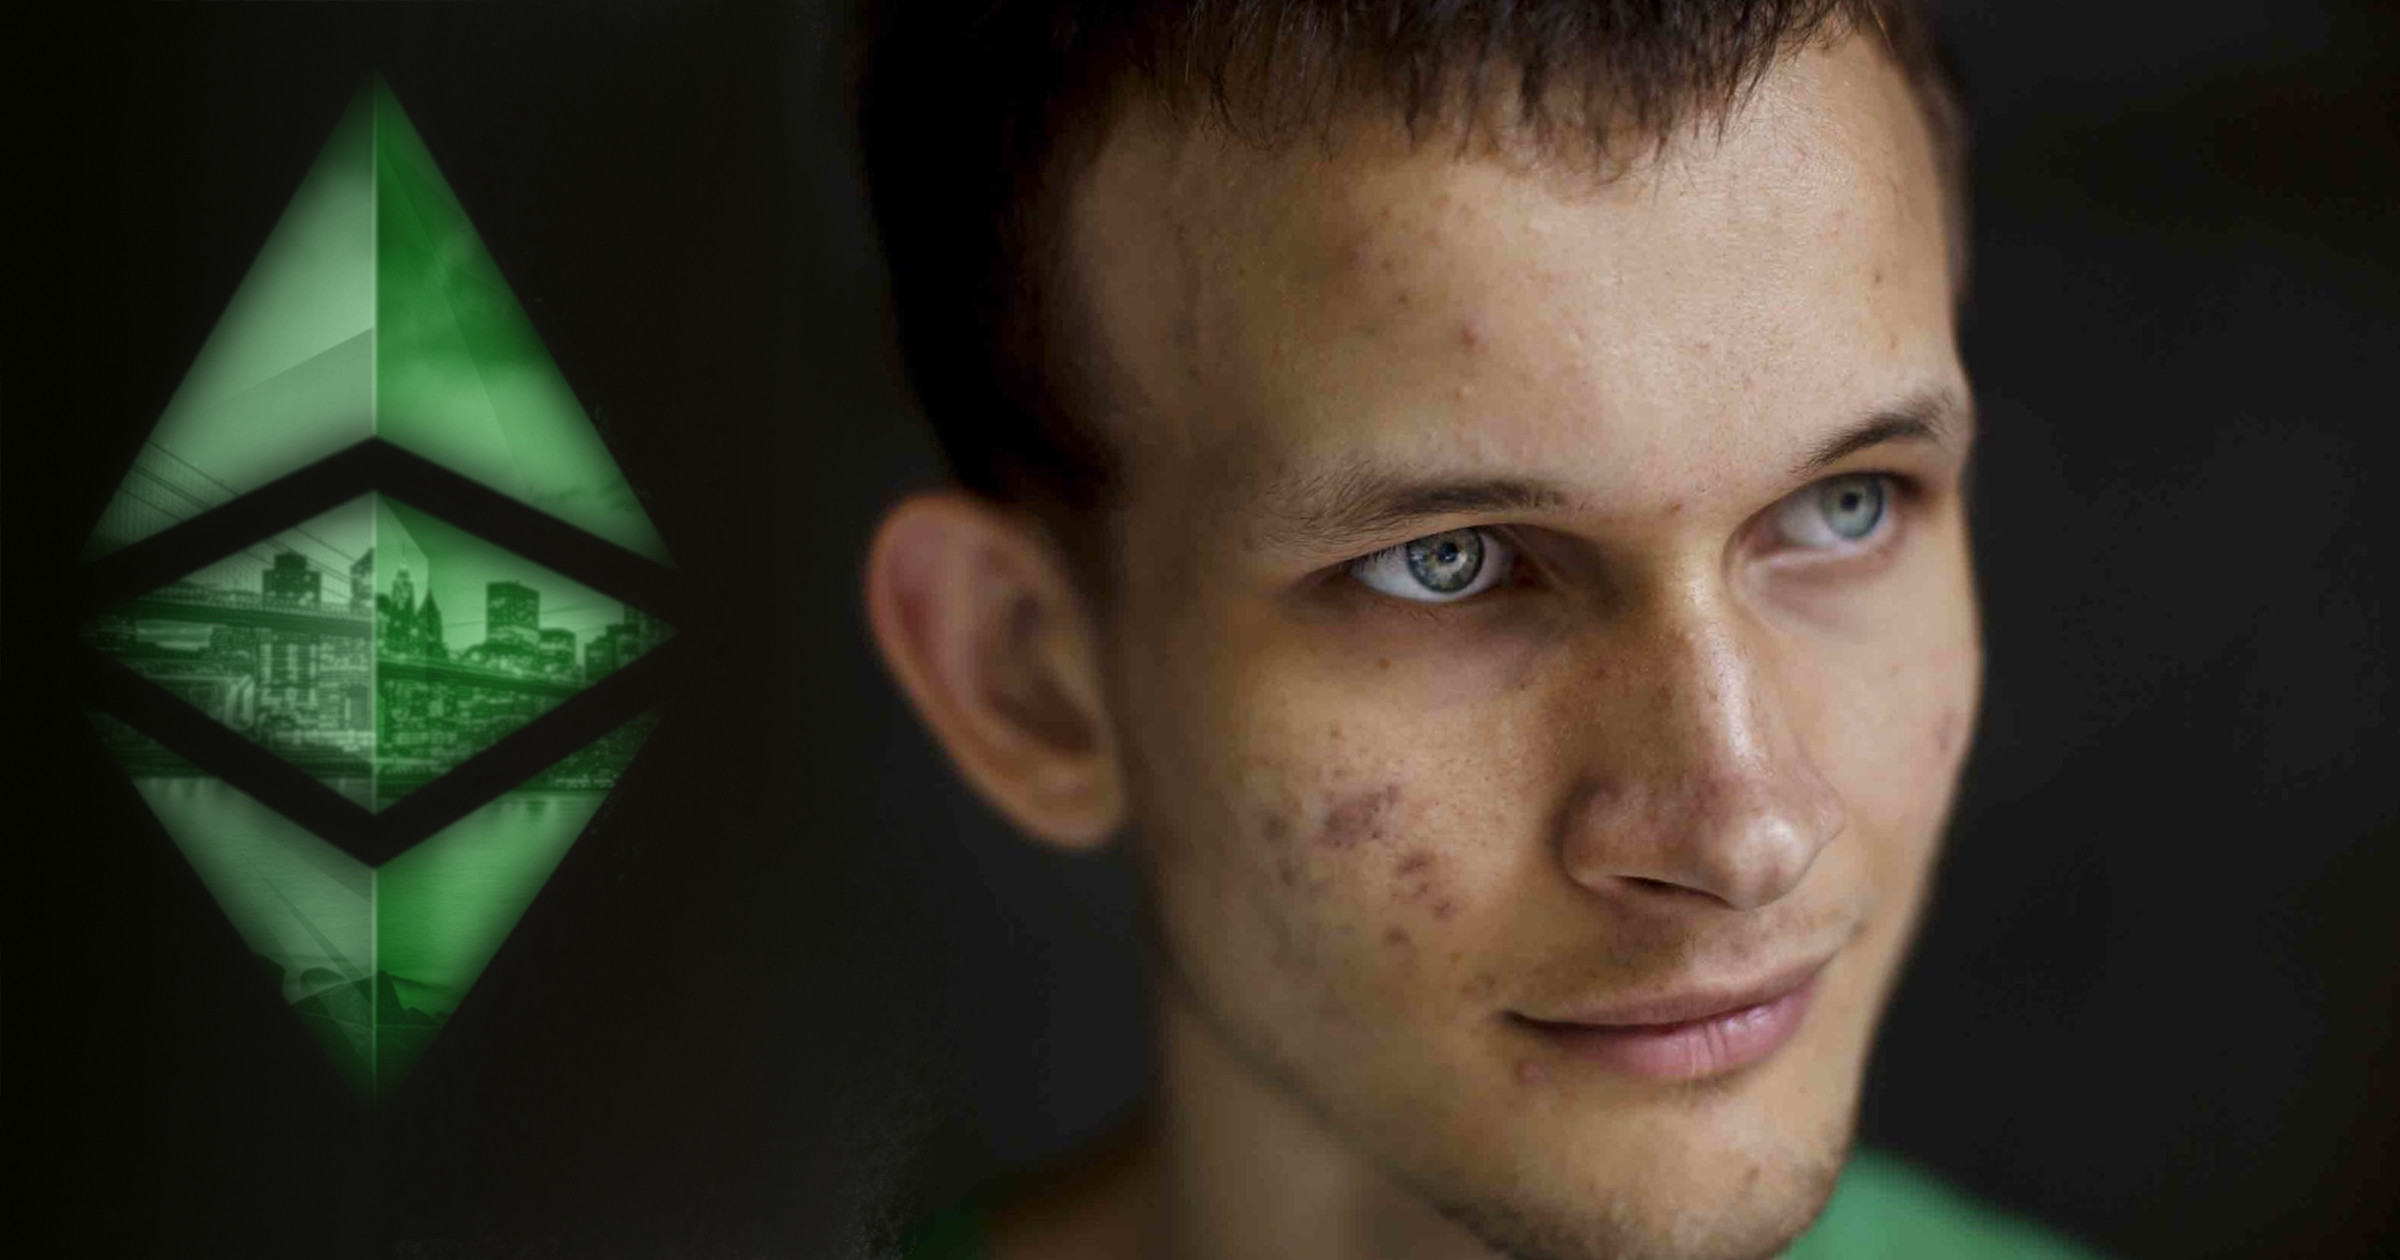
\includegraphics[width=\linewidth]{figures/ethvgod}
				\end{minipage}%
			}
		\end{figure}
	\end{minipage}%
\end{frame}

\begin{frame}{以太坊的理念}
	以太坊是互联网新时代的基础:
	\begin{enumerate}
		\item 内建货币与支付。
		\item 用户拥有个人数据主权,且不会被各类应用监听或窃取数据。
		\item 人人都有权使用开放金融系统。
		\item 基于中立且开源的基础架构,不受任何组织或个人控制。
	\end{enumerate}
\end{frame}

\begin{frame}{比特币和以太坊的关键区别}

	编程语言是否图灵完备\footnote{图灵完备意味着该编程语言可以实现任何逻辑},具备通用计算的能力。

	\begin{table}[htb]
		\label{table:blockchainGeneration}
		\centering
		\begin{tabular}{c|ccc}
			\hline
			             & 区块链1.0 & 区块链2.0 & 区块链3.0 \\
			\hline
			图灵完备     & 否        & 是        & 是        \\
			冯诺伊曼体系 & 否        & 是        & 是        \\
			\hline
		\end{tabular}
		\caption{区块链1.0-3.0的演变}
	\end{table}
\end{frame}

\begin{frame}[allowframebreaks]{区块链1.0:比特币}
	区块链采用纯数学方法而不是中心机构建立信任关系,使得互不信任或弱信任的参与者之间能够维系不可篡改的账本记录。

	具体而言,区块链1.0具有如下功能:
	\begin{itemize}
		\item \textsl{分布式账本(Distributed Ledger)}

		      {\footnotesize 分布式账本是在网络成员之间共享、复制和同步的数据库,记录网络参与者之间的交易。}

		\item \textsl{块链式数据(Linked Data Storage)}

		      {\footnotesize 区块链采用带有时间戳的链式区块结构存储数据,从而为数据增加了时间维度,具有极强的可验证性和可追溯性。}

		\item \textsl{默克尔树(Merkle Trees)}

		      {\footnotesize 梅克尔树是区块链的重要数据结构,能够快速归纳和校验区块数据的存在性和完整性。}

		\item \textsl{工作量证明(Proof of Work, PoW)}

		      {\footnotesize 通过引入分布式节点的算力竞争保证数据一致性和共识的安全性。}
	\end{itemize}
\end{frame}

\begin{frame}[allowframebreaks]{区块链2.0:以太坊}
	区块链2.0进入可编程金融阶段。在这一阶段,区块链系统渗入经济、金融与资本市场,形成股票、债券、期货、贷款、抵押、产权、智能财产的智能合约。

	除了构建货币体系外,区块链在泛金融领域也有众多应用案例。例如,智能合约的核心是利用程序算法替代人执行合同,这些合同包含三个基本要素:要约、承诺、价值交换,可以实现资产、过程、系统的自动组合和项目协调。

	\newpage

	目前,全世界有成千上万名开发者正在以太坊上构建应用程序、发明新的应用程序,其中有许多现在已经可以使用:
	\begin{enumerate}
		\item 	加密货币钱包

		      {\tiny 让你可以使用 ETH 或其他数字资产进行低成本的即时支付;}

		\item 	金融应用程序

		      {\tiny 让你可以借贷、投资数字资产;}
		\item 	去中心化市场

		      {\tiny 让你可以交易数字资产,甚至就现实世界事件的“预测”进行交易;}
		\item 	游戏

		      {\tiny 你可以拥有游戏内的资产,甚至可以由此获得现实收益以及更多,更多。}
	\end{enumerate}
	{\footnotesize 以太坊社区是世界上最大最活跃的区块链社区。它包括核心协议开发者、加密经济研究员、密码朋克、挖矿组织、ETH 持有者、应用开发者、普通用户、无政府主义者、财富 500 强公司。}

	\newpage

	区块链2.0具有如下功能:
	\begin{itemize}
		\item \textsl{智能合约(Smart Contract)}

		      {\tiny 1994 年,Nick Szabo首次提出智能合约概念,即一种旨在以信息化方式传播、验证或执行合同的计算机协议,能够在没有第三方的情况下进行可信交易。智能合约是已编码的、可自动运行的业务逻辑,通常有自己的代币和专用开发语言。}
		\item \textsl{虚拟机(Virtual Machine)}

		      {\tiny 指通过软件模拟的运行在一个完全隔离环境中的完整计算机系统,在区块链技术中,虚拟机用于执行智能合约编译后的代码。}
		\item \textsl{去中心化应用(Decentralized Application, DApp)}

		      {\tiny 去中心化应用是运行在分布式网络上、参与者的信息被安全保护(也可能是匿名的)、通过网络节点进行去中心化操作的应用。包含用户界面的应用,包括但不限于各种加密货币,如以太坊(Ethereum)的去中心化区块链及其原生数字货币以太币(Ether)。}
	\end{itemize}
\end{frame}

\subsection{ICO狂潮和百家争鸣}
\begin{frame}{ICO的含义}
	ICO,全称Initial Coin Offering,意思是“数字货币首次公开募资”。

	概念拷贝自股票市场的IPO,是指企业或非企业组织在区块链技术的支持下发行代币,向投资人募集虚拟货币(一般为比特币、以太坊)的融资活动。

	其流程为:
	\begin{enumerate}
		\item 一家公司或团体表示自己计划或正在研究区块链技术,同时在公有链上内置可转让流通的代币(加密数字货币,与比特币类似);
		\item 投资者以比特币、以太币等虚拟货币换取代币,以此作为其权益凭证;
		\item 项目发行的代币登上交易平台,投资人进行买卖。
	\end{enumerate}
\end{frame}

\begin{frame}{ICO和IPO对比}
	\begin{enumerate}
		\item 共同点:
		      \begin{enumerate}
			      \item 都有通过出售股份来筹措资金;

			      \item 都有潜在投资者为了潜在的巨大收益而冒险参与。

		      \end{enumerate}

		\item 不同点:
		      \begin{enumerate}
			      \item 	ICO的大部分支持者是项目爱好者或不专业的投资者;

			      \item ICO不需要注册经营牌照;

			      \item 	ICO平台是第三方中立平台,投资者自担风险。
		      \end{enumerate}
	\end{enumerate}
\end{frame}

\begin{frame}{ICO狂潮}
	\begin{minipage}[t]{0.4\linewidth}
		\begin{figure}
			\centering
			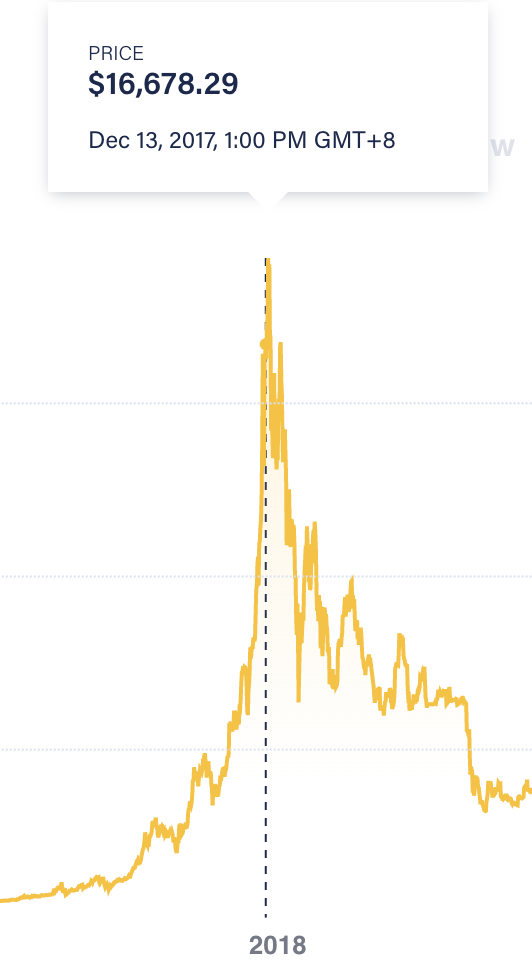
\includegraphics[width=0.7\linewidth,height=0.7\textheight]{figures/94btcprice}
			\caption{\footnotesize 虚拟货币价格达历史峰值}
		\end{figure}
	\end{minipage}%
	\begin{minipage}[t]{0.6\linewidth}
		\begin{table}[]
			\footnotesize
			\begin{tabular}{@{}p{0.1\linewidth}p{0.8\linewidth}@{}}
				\toprule
				时间     & 事件                                                                                       \\ \midrule
				2009     & 比特币上线,区块链慢慢发展;                                                               \\
				2013.7   & Mastercoin(现更名万事达币OMNI)发明ICO;                                                  \\
				2015     & 以太坊上线 ,DAPP概念爆发 ;                                                               \\
				2016.3   & ICO史上最大的众筹项目The DAO,融资额高达1.6亿美元;                                        \\
				2016     & ICO狂潮 ,只要随便写个白皮书都募集到钱;                                                   \\
				2017.9.4 & 比特币价格达到历史峰值,央行联合七部委全面叫停区块链中的ICO事件,同时把ICO定义为非法集资; \\
				2018~   & ICO日渐式微,市场重点转移到区块链与实体经济结合。                                          \\
				\bottomrule
			\end{tabular}
			\caption{ICO大事件}
		\end{table}
	\end{minipage}%
\end{frame}

\section{区块链发展现状:区块链3.0}
\begin{frame}{区块链发展现状:区块链3.0}
	\begin{enumerate}
		\item 政府态度:支持政策大量出台,同时加强监管
		\item 公众普及度:了解但不没用过相关产品
		\item 投资重点:由虚拟货币转向为细分领域
		\item 技术:加速标准化和重要技术突破
	\end{enumerate}
\end{frame}

\subsection{区块链技术发展的关键问题}
\begin{frame}{区块链技术发展的关键问题}
	\begin{enumerate}
		\item \textbf{性能问题}

		      指的是区块链的每秒交易量和交易延迟无法满足上层应用的问题;

		\item \textbf{存储问题}

		      指的是区块链的数据存储空间无法满足目前区块链应用的存储需求的问题;

		\item \textbf{隐私安全问题}

		      指的是在开放的区块链环境中如何保护区块链用户数据隐私的问题。
	\end{enumerate}
\end{frame}

\subsection{区块链细分技术成熟度}
\begin{frame}{区块链细分技术成熟度}
	\begin{figure}
		\centering
		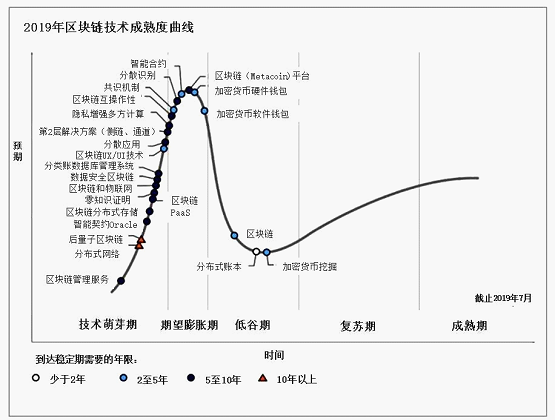
\includegraphics[width=0.7\linewidth]{figures/2019区块链成熟度曲线}
		\caption{2019区块链成熟度曲线}
		\label{fig:2019blockchainpostion}
	\end{figure}
\end{frame}

\subsection{区块链目前的主要研究内容}
\begin{frame}{目前主要工作是突破区块链基础技术}
	目前主要工作是改善区块链的可伸缩性、隐私性、数据存储、互操作性、托管和用户体验
	\begin{figure}
		\centering
		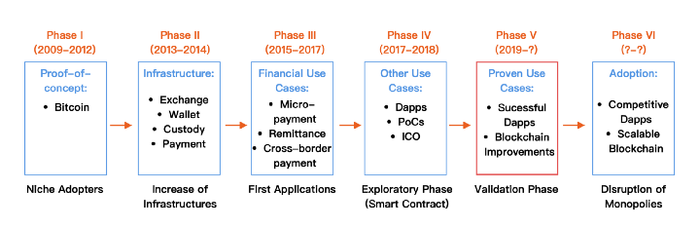
\includegraphics[width=0.9\linewidth]{figures/blockchainsteps}
		\caption{区块链发展阶段}
		\label{fig:blockchainsteps}
	\end{figure}

\end{frame}

\begin{frame}{区块链性能进展}
	\begin{enumerate}
		\item \textbf{部分中心化方案}

		      {\scriptsize 通过部分中心化的方式提高共识效率、降低节点账本存储压力;}

		\item \textbf{双层方案}

		      {\scriptsize 	将区块链解构成两层,第一层(Layer 1)保证区块链的安全性,第二层(Layer 2)将不相关的交易分散到不同的子域进行处理,极大提高了区块链的性能。}
		      \begin{enumerate}
			      \item  \textbf{有向无环图} (DAG)

			            {\scriptsize 将区块链的出块方式由链式解构变为有向无环图解构,异步和并发出块从而提高性能;}
			      \item  \textbf{分片} (Sharding)

			            {\scriptsize 将将需要处理的交易分摊给多组参与共识的节点进行处理,并发交易处理从而提高性能;}

			      \item  \textbf{跨链} (CrossChain)

			            {\scriptsize 将需要处理的交易分摊给不同的子链进行处理,异步和并发出块从而提高性能;}
		      \end{enumerate}
	\end{enumerate}
\end{frame}

\begin{frame}{区块链存储进展}
	可靠的、去中心化的、可验证的存储能力需求在区块链的发展中愈发迫切。目前,基于P2P技术和云存储技术的区块链存储技术,例如 IPFS \& FileCoin 、Sia、Swarm、Storj、MaidSafe,已经可以满足区块链存储的基本要求。但是其与区块链技术的融合仍然存在着诸多问题:

	\begin{enumerate}
		\item \textbf{存储系统的经济模型问题}

		      {\scriptsize  是指通过区块链通证技术和区块链存储系统的有机结合,构建一个用以维护区块链存储系统稳定运行、刺激网络用户存储能力的经济模型问题。当前还未出现完美解决方案。对新节点加入的筛选机制,对于节点的安全性、可靠性,加入节点后如何持续提供稳定、可靠的存储能力,是需要未来系统设计时考虑的;}
		\item \textbf{存储空间的证明问题}

		      {\scriptsize  是指如何通过某种证明机制向其他节点证明自己确实存储了某一项数据的证明问题。存储证明是区块链存储的主要特征,是将存储与区块链通证结合的关键,是项目方结合自身的业务模型和经济模型设计的,为了激励节点贡献存储能力的必要手段;}
		\item \textbf{数据的隐私问题}

		      {\scriptsize  是指如何保护用户存储在区块链存储系统中的数据隐私问题。}
	\end{enumerate}
\end{frame}

\begin{frame}{区块链隐私安全进展}
	区块链的去中心化特性和公开透明的数据对用户隐私带来了挑战。在不破坏区块链安全性的前提下完成去中心化的区块链隐私和安全保护成为区块链隐私安全的重要研究课题。

	\begin{enumerate}
		\item \textbf{零知识证明} (Zero-Knowledge Proof)

		      {\scriptsize 指的是一种证明者能够在不向验证者提供任何有用信息的情况下,使验证者相信某个论断是正确的的方法;}

		\item \textbf{可信执行环境} (TEE, Trusted Execution Environment)

		      {\scriptsize 	指的是在硬件设备上提供一个隔离的安全执行空间(TrustZone),使得所有需要保密的操作可以在可信的环境中执行(例如密码处理、数据加解密、安全认证等),使得区块链可以弱化其安全模型。目前TEE主要依赖芯片厂商的支持,如ARM、英特尔等;}

		\item \textbf{安全多方计算} (MPC, Secure Muti-party Computation)

		      {\scriptsize 	指的是一种允许多个数据所有者在互不信任的情况下进行协同计算,输出计算结果,并保证任何一方均无法得到除应得计算结果之外的任何信息。换句话说,MPC技术可以获取数据使用价值,却不泄露原始数据内容。}
	\end{enumerate}
\end{frame}

\subsection{政府加强区块链监管}
%%%%%%%%%%%%%%%%%%%%%%%%%%%%%%%
% 注释:
%% 区块链是一项全新的信息技术,将影响甚至颠覆很多产业业态、商业模式以及管理制度,推动目前的信息互联网升级成价值互联网。其近年来得到诸多国家、机构和个人的重视 。不过,和互联网与信息技术不同,比特币及其所依托的底层技术区块链在产生伊始,即自带金融风险,从技术或价值上来看,并非完全中立的,或者说,区块链技术存在较为典型的价值观偏向。在这种价值观指引下,区块链应用场景多为金融以及信用缺失的领域,具体包括数字货币、众筹、清算、结算与审计、智能合约、版权与许可、公证与记录等。近年一份白皮书亦指出,区块链已成为金融科技发展最重要的一种信息技术,区块链最早的应用领域、区块链应用项目数量最多、区块链应用程度最深的领域也是金融服务。因此,区块链在银行、支付、票据、证券、保险和会计审计等金融相关领域得到非常广泛的运用。自2009年以来,区块链技术尤其在虚拟货币、虚拟货币交易所和首次代币发行(ICO)领域,孕育着巨大金融风险 。仅在比特币领域,研究者认为,其带来的风险就包括便利黑色市场交易、避税、洗钱以及恐怖主义融资等。因此有必要对区块链技术及应用进行适当的监管
%%%%%%%%%%%%%%%%%%%%%%%%%%%%%%%%%
\begin{frame}{区块链监管的必要性}
	\begin{enumerate}
		\item  保护投资者的需要
		\item  维护全行业合法性的需要
		\item 保证高质量代币发行的需要
	\end{enumerate}
\end{frame}
\begin{frame}{区块链对监管带来的压力}
	\begin{enumerate}
		\item 虚拟货币法律定性的欠缺
		\item 区块链的跨区域性造成管辖权冲突
		\item 区块链的去中心化导致责任主体不明确
		\item 区块链的复杂性与快速传播特性使得风险管理难度大
	\end{enumerate}
\end{frame}

\subsection{区块链标准化加速}
\subsubsection{标准化的益处}
\begin{frame}{标准化的益处}

	\begin{enumerate}
		\item \textbf{对企业利好}

		      {\scriptsize 标准是解决区块链商业化应用过程中面临最大挑战的战略工具和指南,并能确保业务高效运营,提高生产率和帮助企业拓展新的市场;}

		\item \textbf{对用户利好}

		      {\scriptsize 区块链相关的产品和服务符合标准,意味着是安全的、可靠的和高质量的;}

		\item \textbf{对政府利好}

		      {\scriptsize 标准是制定政策和加强市场监管的重要依据,对提高政策水平和对外开放水平,具有重要作用。	}
	\end{enumerate}
\end{frame}
\subsubsection{全球加强区块链标准化进程}
\begin{frame}{全球加强区块链标准化进程}
	\begin{table}[]
		\footnotesize
		\begin{tabular}{p{0.1\textwidth}p{0.75\textwidth}}
			\toprule
			时间       & 节点                                                                                                                                                            \\ \midrule
			2016.4     & 由澳大利亚标准公司牵头,将关于区块链国际标准化的提议提交给国际标准化组织(ISO)。                                                                                 \\
			2016.9.15  & 澳大利亚标准公司的提议获得ISO通过,“区块链和分布式账技术标准化技术委员会”(ISO/TC 307)正式成立,澳大利亚标准公司成为当中的秘书处,主导创建统一的区块链技术方法。 \\
			2017.3.2   & 澳大利亚标准公司公布了《区块链标准路线图》,组织成员国关于区块链标准的开发将在“区块链和分布式账技术标准化技术委员会”(ISO/TC 307)的监督下进行。                  \\
			2017.4.3   & 国际标准化组织(ISO)区块链和分布式分类帐技术标准化技术委员会(ISO/TC 307)在澳大利亚悉尼举行第一次全体会议。                                                       \\
			2017.11.13 & 国际标准化组织(ISO)区块链和分布式分类账技术标准化技术委员会ISO/TC 307 在日本东京举行第二次全体会议。                                                            \\
			2018.5.14  & 国际标准化组织(ISO)区块链和分布式分类帐技术标注啊技术委员会ISO/TC 307 在英国伦敦举行第三次全体会议。                                                            \\
			\bottomrule
		\end{tabular}
		\caption{区块链标准化组织 ISO/TC 307成立时间表}
		\label{tab:ISOTC307}
	\end{table}
\end{frame}

\subsubsection{中国加强区块链标准化进程}

\begin{frame}[allowframebreaks]{中国加强区块链标准化进程}
	\tiny
	\begin{table}[]
		\begin{tabular}{p{0.1\textwidth}p{0.6\textwidth}}
			\toprule
			时间       & 节点                                                                                                                                                                                                                                                                          \\ \midrule
			2016.7     & 印发了《关于组织开展区块链技术和应用发展趋势研究的函》(工信部软函{[}2016{]}840号),委托工信部电子标准院联合蚂蚁金服、万向控股、微众银行和平安保险等国内重点企业开展区块链技术和应用发展趋势研究工作。                                                                         \\
			2016.8     & 8月5日,召开了区块链技术和产业发展论坛筹备会暨白皮书编写启动会。中国电子技术标准化研究院开展“十问区块链”专题研究,设计去中心化、应用模式、信息安全挑战等热点问题。                                                                                                            \\
			2016.10.18 & 由工信部、国家标准化管理委员会指导的“中国区块链技术和产业发展论坛”宣布在北京成立。同期发布的《中国区块链技术和应用发展白皮书(2016)》中,提出了区块链标准化路线图和标准体系框架。(*中国电子技术标准化研究院担任中国区块链技术和产业发展论坛的理事长单位,论坛秘书处挂靠研究呀) \\
			2017.4     & 中国代表团参加了ISO/TC 307 成立以来的第一次全体会议。中国代表团主要介绍了《中国区块链技术和应用白皮书(2016)》和《区块链参考架构》两项工作成果。同时,建议成立术语和参考架构工作组,并申请委派专家担任工作组召集人职务,承担后续标准研制工作。                                 \\
			\bottomrule
		\end{tabular}
		\caption{中国的区块链标准化之路1}
	\end{table}%
	\begin{table}[]
		\begin{tabular}{p{0.1\textwidth}p{0.6\textwidth}}
			\toprule
			时间       & 节点                                                                                                                                                                                                                                      \\ \midrule
			2017.5.14  & 在杭州萧山(G20峰会)举办了首届区块链开发大赛,征集到区块链技术应用方案58份,对《区块链参考架构》起到了良好的验证作用,16日,发布《区块链参考架构》标准,同时基于该标准开发了《区块链系统功能测试方案》,并完成对12家机构的系统进行的测试。 \\
			2017.8     & 拟定了《中国区块链技术和产业发展论坛开源社区章程》                                                                                                                                                                                        \\
			2017.11    & ISO/TC 307第二次全体会议,中国等20多个国家参与制定《ISO/TC 307区块链国际标准》,中国的《区块链参考架构》为此项工作做出了重要贡献。                                                                                                        \\
			2017.12.22 & “中国区块链技术和产业发展论坛第二届开发大会”在广州市萝岗召开,会上同时发布了论坛的第二个标准《区块链数据格式规范》。                                                                                                                      \\
			2018.3.12  & 为做好ISO/TC 307在国内的技术对口工作,工信部软司指导电子标准院提出全国区块链和分布式记账技术标准化委员会组件方案。                                                                                                                        \\
			2018.6.20  & 工信部科技司公示“全国区块链和分布式记账技术标准化技术委员会筹建方案”。                                                                                                                                                                    \\
			\bottomrule
		\end{tabular}
		\caption{中国的区块链标准化之路2}
	\end{table}
\end{frame}

\subsection{区块链和互联网的对比}
\begin{frame}{区块链发展类似互联网,且仍然处于早期}
	区块链正在爆发式发展,其市场是互联网的10倍。
	\begin{figure}
		\centering
		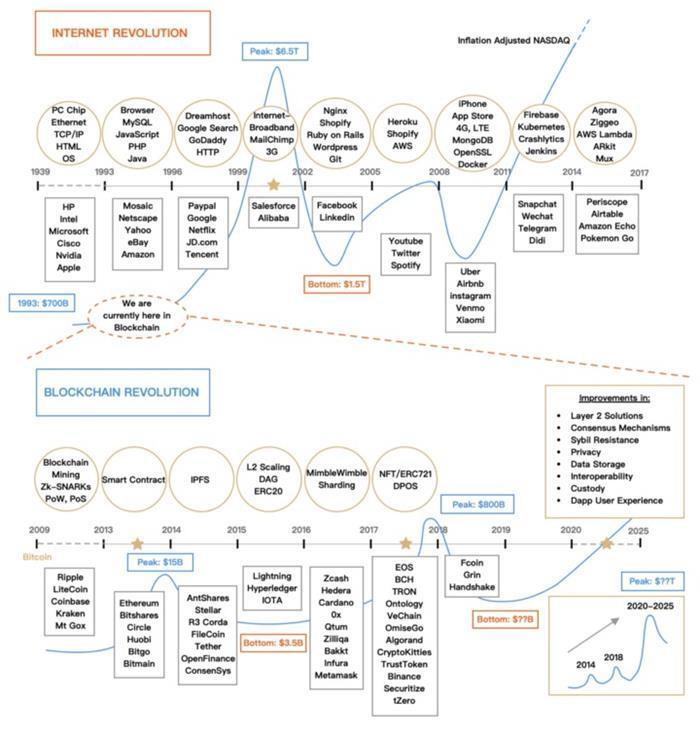
\includegraphics[width=0.8\linewidth,height=0.6\textheight]{figures/blockchainrevelution}
		\caption{互联网和区块链历程与对比}
		\label{fig:blockchainrevelution}
	\end{figure}
\end{frame}

\begin{frame}{区块链用户数预测}
	\begin{figure}
		\centering
		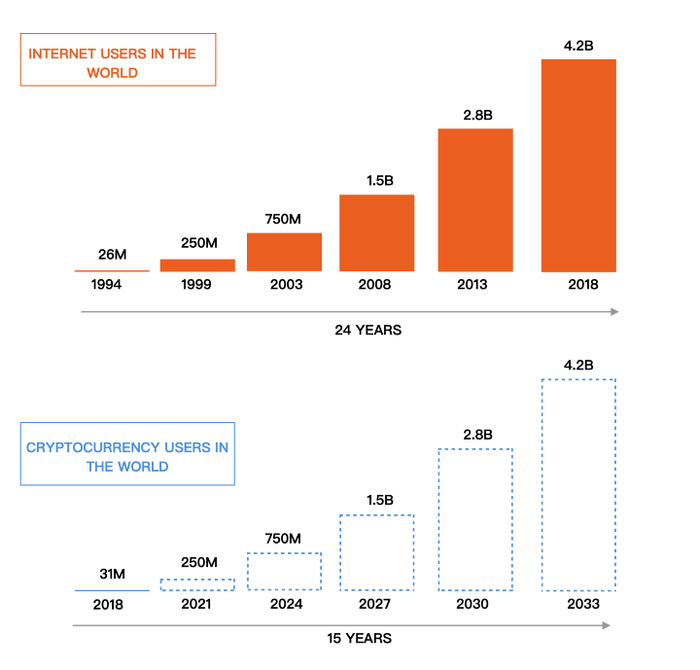
\includegraphics[width=0.7\linewidth, height=0.7\textheight]{figures/compareinternetandblockchain}
		\caption{互联网和区块链用户数预测}
		\label{fig:compareinternetandblockchain}
	\end{figure}

\end{frame}


% 我们目前正在过渡到区块链演进的第五个阶段,在这个阶段中,区块链在不同行业的应用以及区块链可扩展性解决方案正在被探索。在第一阶段,2009-2012年,比特币作为一种新型的数字货币和概念验证发布,第一批用户由核心技术人员、加密专家和密码朋克组成,他们在各种邮件列表和论坛(bitcointalk.org、Reddit等)上推广加密货币。2013-2014年第二阶段,随着媒体报道的增加(虽然很多是负面报道),交易所、钱包、托管、支付解决方案等基础设施开始增加。2015-2017年第三阶段更侧重于围绕金融用例的实际应用,如汇款、小额支付、跨境支付。随着以太坊的智能合约的出现,我们已经进入了第四个阶段,在这个阶段中,我们正在探索金融之外的用例,而新的融资工具ICO在这个阶段成为了一个杀手应用程序。在第五阶段,我们期待着成功的DAPP和用例的出现,重新树立对技术的信心,改善区块链的可伸缩性、隐私性、数据存储、互操作性、托管和用户体验。在第六阶段的后期,我们希望看到DAPP打破并与Dropbox、Facebook、Youtube、Airbnb等集中式垄断企业竞争,让消费者参与到数字经济中,并获得更多的权利。

\subsection{区块链应用领域一览}
\begin{frame}[allowframebreaks]{区块链应用领域一览}
	\begin{figure}
		\centering
		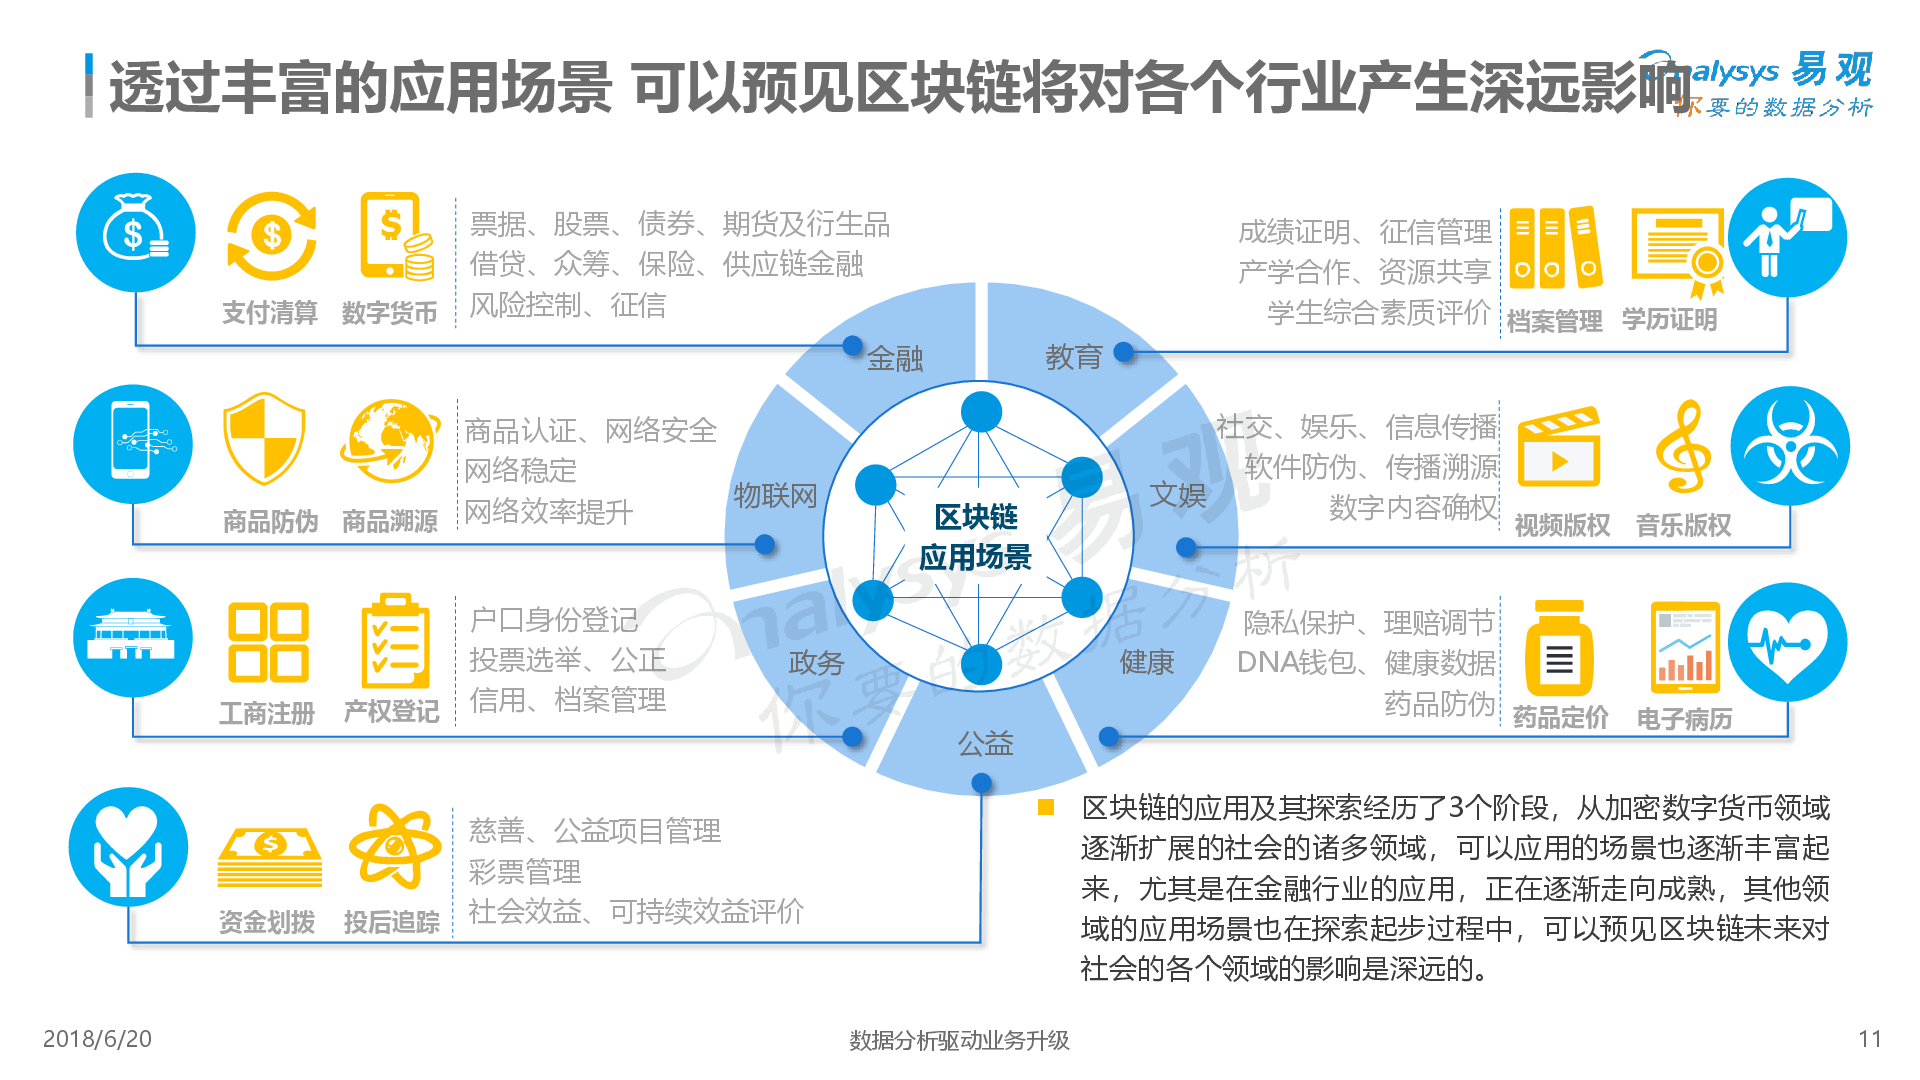
\includegraphics[width=0.9\linewidth]{figures/blockchainapplications}
		\label{fig:blockchainapplications}
	\end{figure}

	\begin{figure}
		\centering
		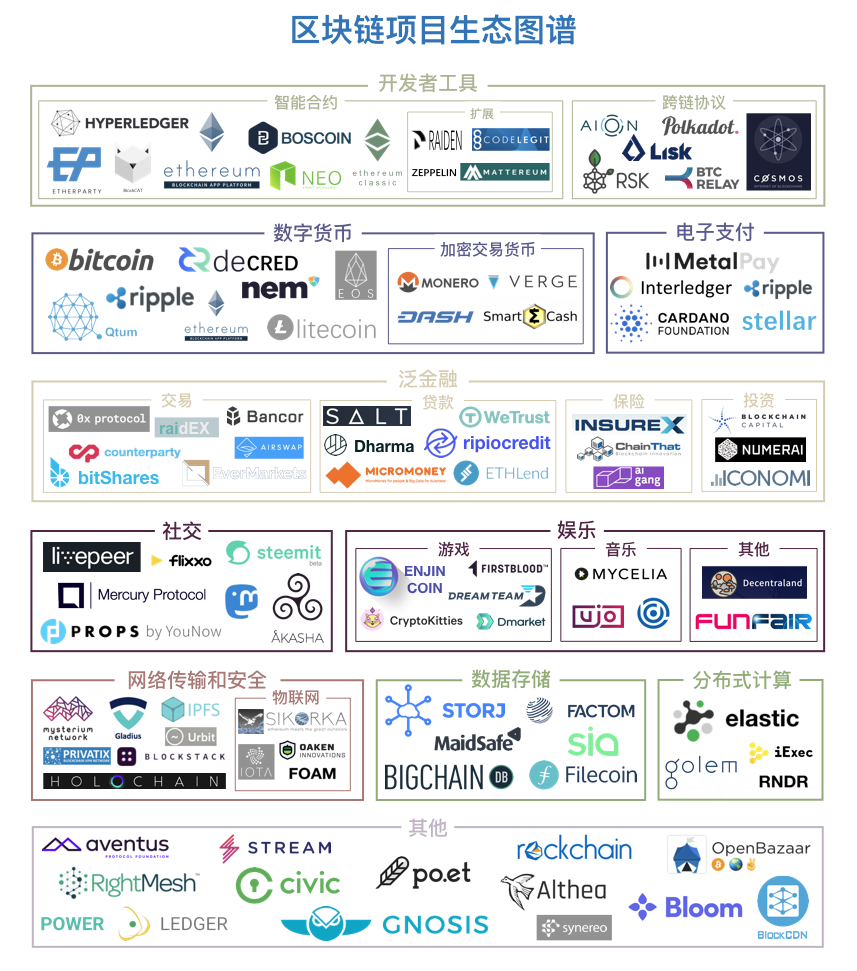
\includegraphics[height=0.85\textheight]{figures/blockchainenv}
		\label{fig:blockchainenv}
	\end{figure}
\end{frame}

\subsection{区块链相关企业一览}

\begin{frame}[allowframebreaks]{区块链相关企业一览}
	\begin{figure}
		\centering
		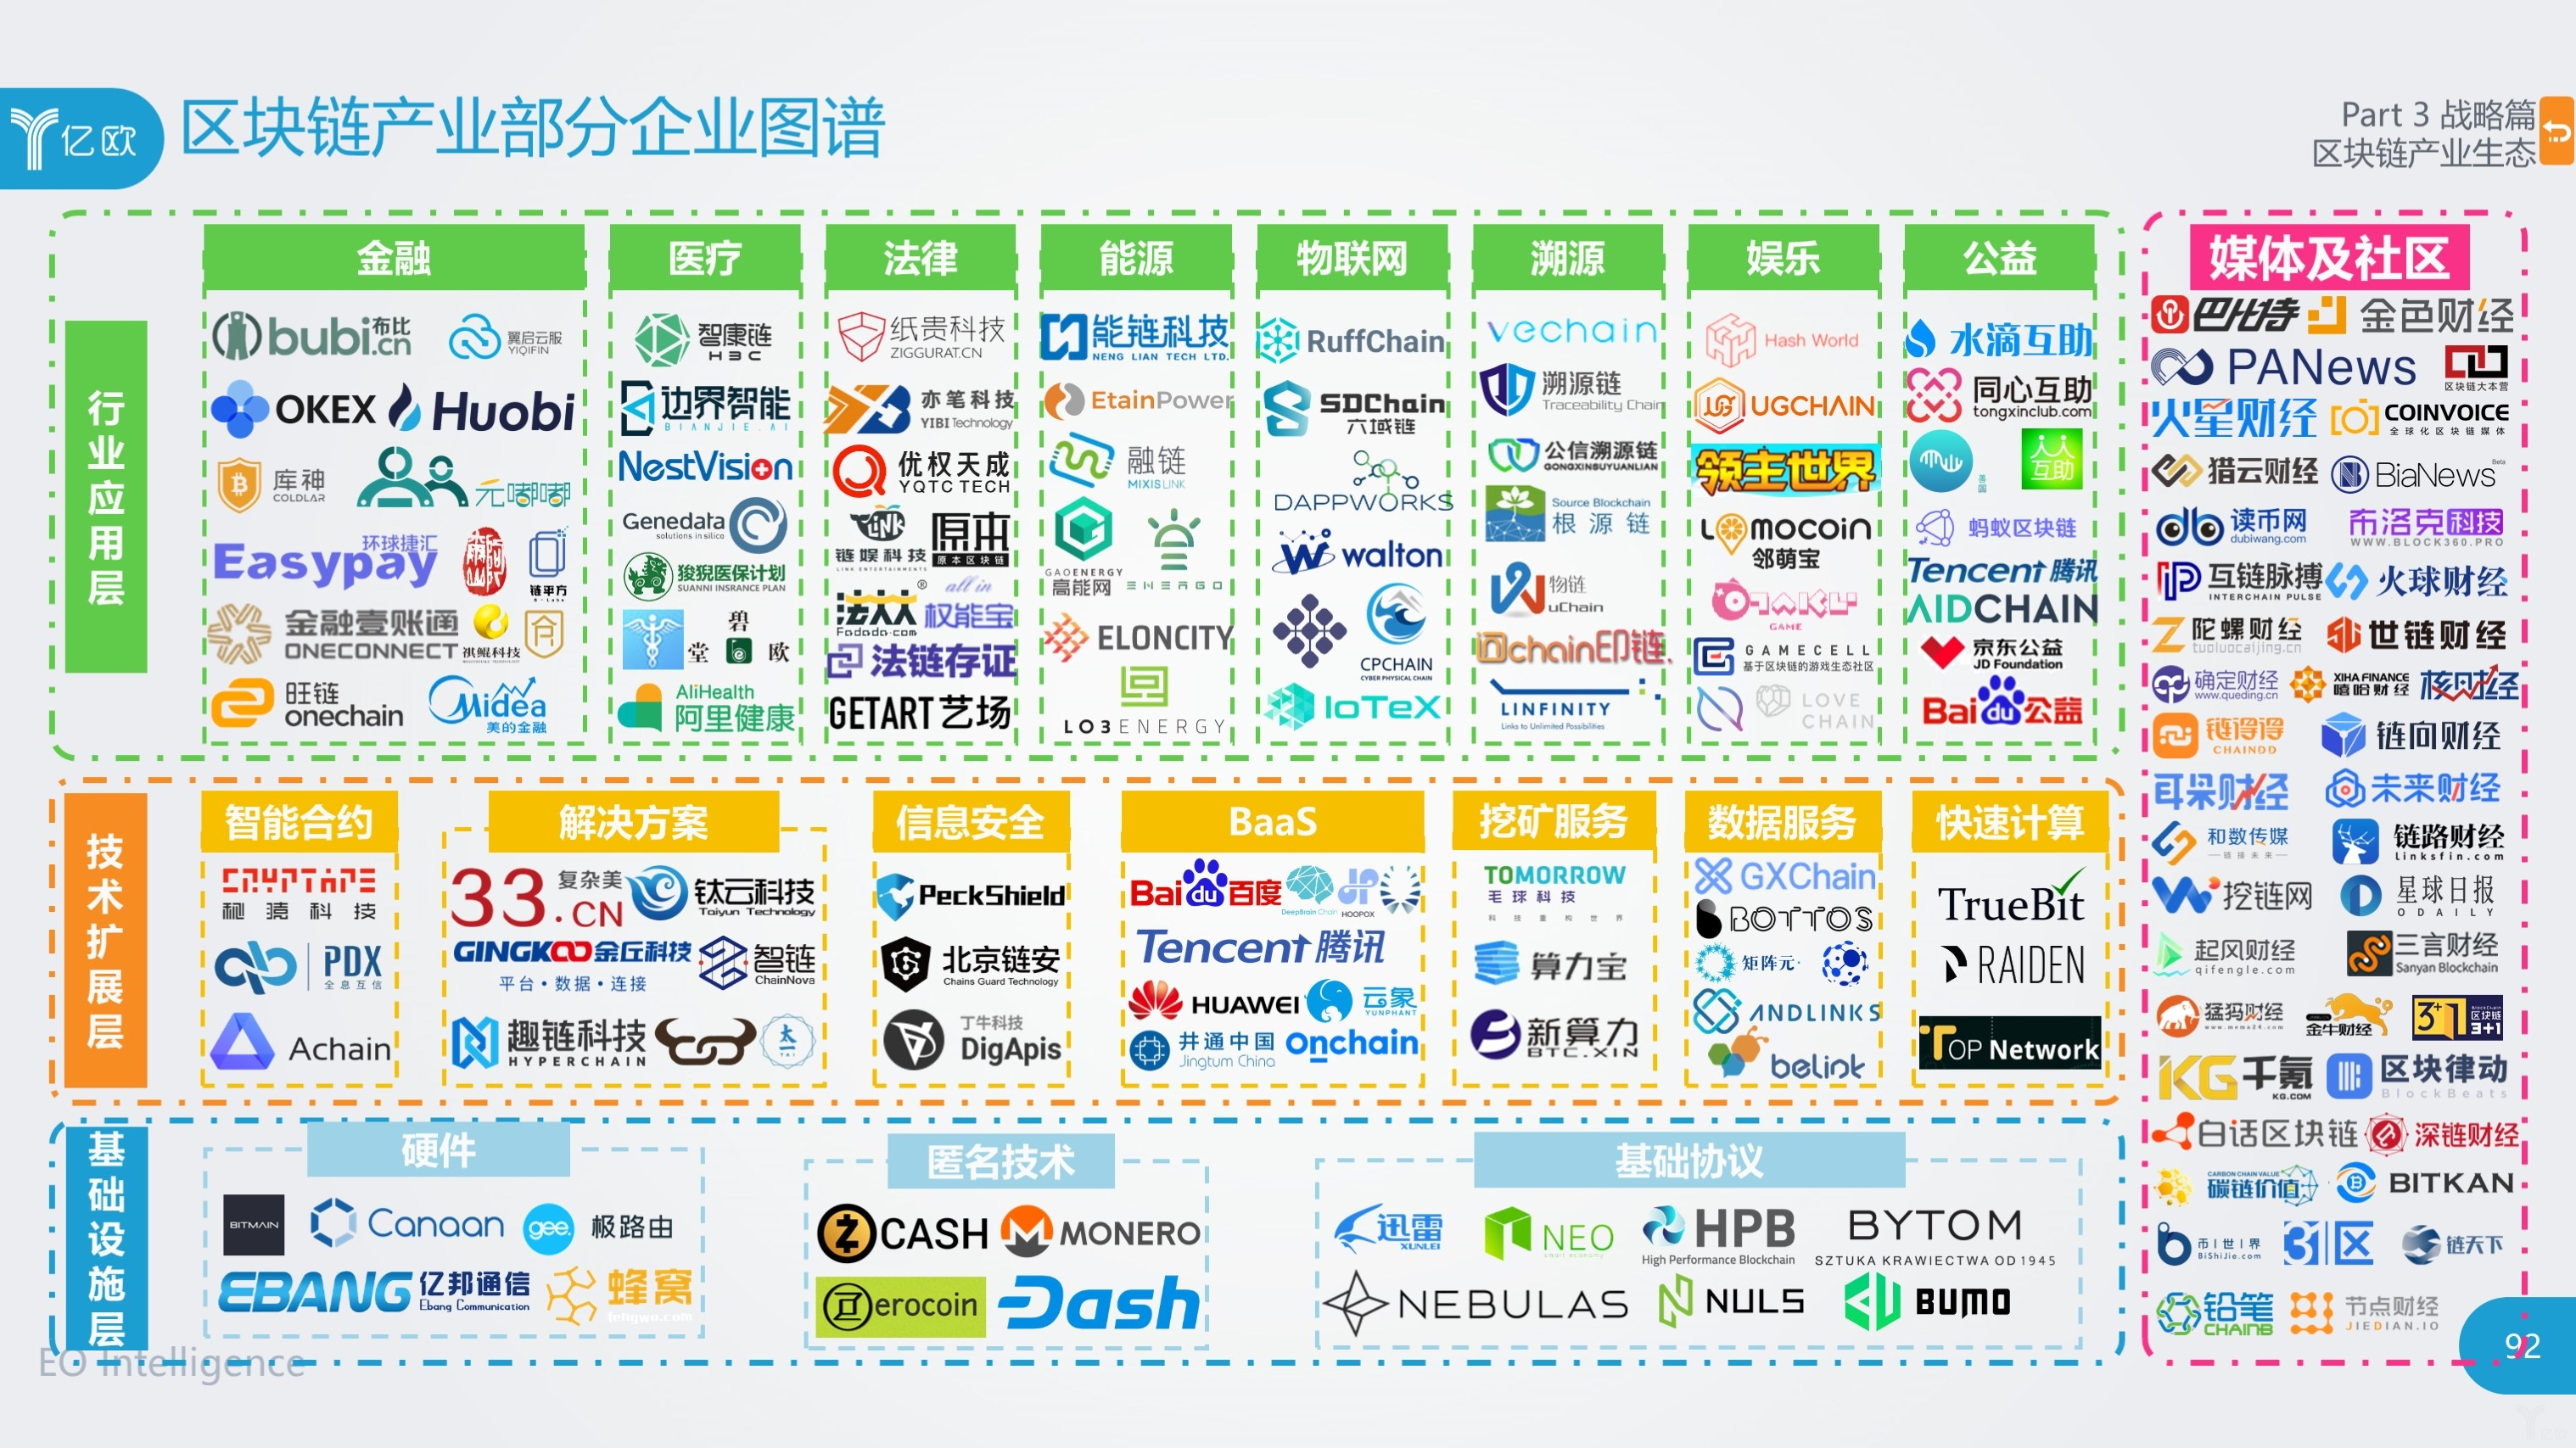
\includegraphics[width=0.9\linewidth]{figures/chinablockchaincompany}
		\label{fig:chinablockchaincompany}
	\end{figure}
	\begin{figure}
		\centering
		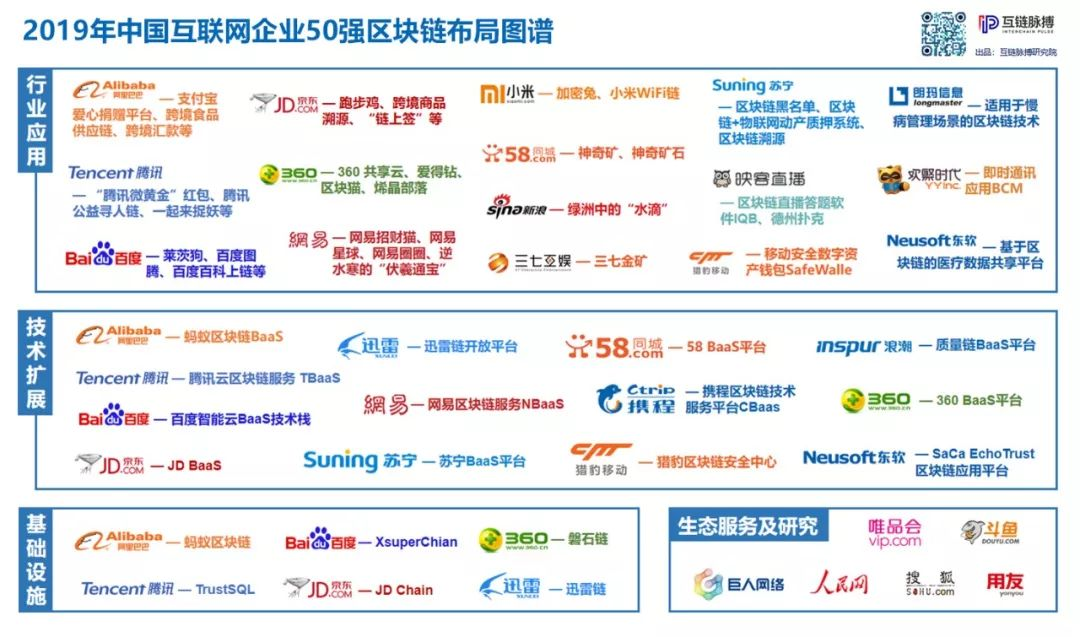
\includegraphics[width=0.9\linewidth]{figures/chinabigcompnayinblockchain}
		\label{fig:blockchainconpanyinchina}
	\end{figure}
	\begin{figure}
		\centering
		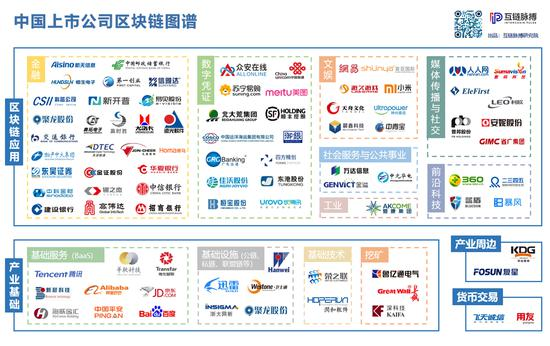
\includegraphics[width=0.9\linewidth]{figures/bigcompany2}
		\label{fig:bigcompany2}
	\end{figure}

\end{frame}

\section{重要提示}
\begin{frame}{勿当韭菜!!!别碰加密货币!!!}

	{\color{red}
		数字货币骗子口头禅大赏:
		\begin{itemize}
			\item 发币前许你美景:MIT、JP摩根团队;价值投资;一币一别墅;
			\item 发币后叫你稳住:团队在做事;拿住;价值投资;
		\end{itemize}
	}
	\begin{figure}
		\centering
		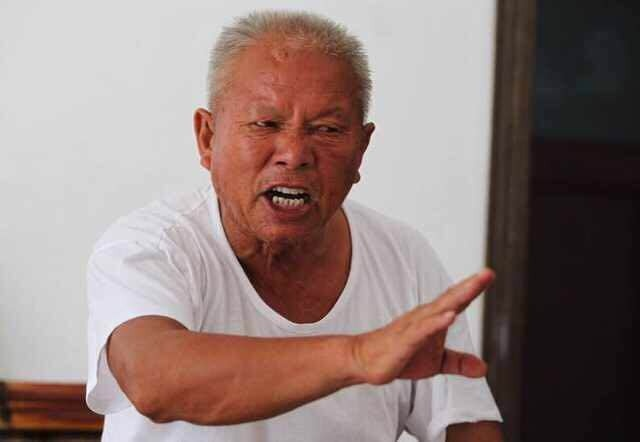
\includegraphics[width=0.5\linewidth]{figures/AllInGrandpa}
		\caption{什么团队背景,什么技术方案,老夫选币都是一把梭.mp4}
		\label{fig:allingrandpa}
	\end{figure}

\end{frame}

\section*{谢谢聆听}

\begin{frame}
	\begin{minipage}[t]{0.5\linewidth}
		\begin{center}
			\begin{figure}
				\vspace{10pt}
				
				{\Huge 谢谢聆听}
				
				\vspace{30pt}
				郭泰彪
				
				\vspace{10pt}
				{\tiny 湖南工商大学大数据与互联网创新研究院}
			\end{figure}
			\begin{figure}
				
			\end{figure}
		\end{center}
	\end{minipage}%
	\begin{minipage}[t]{0.4\linewidth}
		\begin{figure}
			\centering
			\texttt{blockchain101}
			
			
\includegraphics[width=0.6\linewidth]{figures/blockchain101qrcode}
			
			{\footnotesize \texttt{Star| Fork| Issue}}
		\end{figure}
	\end{minipage}%
\end{frame}

\end{document}